% !BIB TS-program = biber
%--------------------
% Packages
% -------------------
\documentclass[11pt,a4paper]{article}

\usepackage{mathptmx} % Use Times Font
\usepackage{times}
\usepackage{amsmath}
\usepackage[UKenglish]{babel}
\usepackage[style=authoryear,backend=biber,uniquename=false,maxnames=2,minnames=1]{biblatex} %Imports biblatex package
\usepackage{csquotes}
\usepackage{placeins}
\usepackage{afterpage}
\addbibresource{ref.bib}
\usepackage[pdftex]{graphicx} % Required for including pictures
\usepackage[pdftex,linkcolor=black,pdfborder={0 0 0}]{hyperref} % Format links for pdf
\usepackage{calc} % To reset the counter in the document after title page
\usepackage{enumitem} % Includes lists
\usepackage{booktabs}
\frenchspacing % No double spacing between sentences
\linespread{1.2} % Set linespace
\usepackage[a4paper, lmargin=0.1666\paperwidth, rmargin=0.1666\paperwidth, tmargin=0.1111\paperheight, bmargin=0.1111\paperheight]{geometry} %margins
%\usepackage{parskip}

\usepackage[all]{nowidow} % Tries to remove widows
\usepackage[protrusion=true,expansion=true]{microtype} % Improves typography, load after fontpackage is selected




%-----------------------
% Set pdf information and add title, fill in the fields
%-----------------------

\title{Attribution of the  extreme precipitation related to Derailment  on August 12th 2020 in Carmont, Scotland}
\author{Simon F. B. Tett\thanks{School of Geosciences, University of Edinburgh, Edinburgh EH9 3JW, UK} \thanks{CLXX, UNSW, Sydney, NSW, XXXX, Australia}
	\and 
Chris Long\thanks{School of Physics, University of Edinburgh, Edinburgh EH9 xxx, UK}
\and 
ANY MORE\thanks{Address}}


%-----------------------
% Begin document
%-----------------------

\begin{document}
	
\maketitle

\graphicspath{{../figures/}}


\begin{abstract}

	The UK's Convective Permitting Model suggests, in the Stonehaven area, that extreme hourly rainfall changes at Clausius–Clapyron +50\%. This leads to an increased probability, relative to late 19th century conditions,  of rainfall similar to the rain that was associated with the fatal rail accident in Carmont on August 12th 2020, by about 30\% with a doubling of probability for such events in a +2K warmer world. Some characteristics of the simulated extreme rain evaluate well against radar values but the  simulated rainfall is about 20-30\% larger than the radar rainfall. This may reflect model problems or shortcomings in  radar  calibration. 
\end{abstract}



\section{Introduction}
\label{sect:Intro}

On August 12th 2020 a passenger train running from Aberdeen to Glasgow derailed at Carmont near Stonehaven. The train was lightly loaded due to COVID restrictions. Even so,  three people died and the remaining six people on the train  were injured. The proximate cause of the derailment was gravel being washed out of a drain \parencite{carmontReport2024}. Radar estimates of  rain at 1km x 1km resolution was 51.5 mm of rain falling between 05:50 to 09:00 which was estimated at around a 1-in-a-100 year event. The drain should have been able to deal with that volume of water but because the drain had not been built to design requirements gravel and other debris was washed out of it and onto the tracks. This in turn caused the derailment. In the aftermath of the derailment UK Government commissioned a report to examine the resilience of the UK's rail infrastructure\parencite{NR_DfT_2021}. It reported that the signal of climate change is becoming more significant  also examined the impacts of future climate change  on rail infrastructure.


 Serious accidents often require several things to go wrong. In the case of Carmont derailment  the both a not to specification drain construction and extreme rainfall were required. This paper focuses on the rainfall component of the accident. It develops methodology to estimate, from radar data, the return period of the radar rain, uses convective permitting model (CPM) simulations to estimate how climate change (largely anthropogenic) has changed the distribution of extreme precipitation at Carmont. Finally we adjust the radar estimated distribution by the CPM changes to provide an event attribution of the extreme rainfall. 

Theory\parencite{allen02insight} suggests that extreme rainfall occurs when the entire column of atmospheric water precipitates. This, in turn,  suggests that extreme precipitation increases fractionally at the same rate as saturated humidity, or for fixed atmospheric pressure, saturated vapour pressure (Clausius-Clapyron; CC). This is about 7\%/K. However,  studies suggest that sub-daily extreme rainfall  could increase  at rates  up to twice CC\parencite{fowler2021rainfall_extremes} with a clear signal in both observations and CPM relating contemporaneous dew-point temperature to extreme rainfall. 

The last IPCC report\parencite{Seneviratne2021ippcc_chapter_extremes} reported on the lack of systematic analysis of long-term trend in sub-daily extreme precipitation at global scales (Sect 11.4). Though, did report on regional studies that found intensification at those scales. It also criqued the apparent scaling of sub-daily precipitation extremes. There has  been an extremely limited number of studies that attempted to attribute changes in sub-daily extreme rainfall, with none reported in \cite{Seneviratne2021ippcc_chapter_extremes},  though several studies have attributed changes in daily or longer time-scale rainfall\parencite{clarke2022extreme_Attribution,Zhang2020rainfall,tradowsky2023w_europe_rain}.  Studies that attempted to attribute changes in sub-daily extreme precipitation are \cite{mishra2023landslide} who used  data from a CPM simulation of a storm in 2009 and with pre-industrial conditions found that changes in three-hourly extremes had increased the frequency of landslides by about 10\%. While \cite{Reed2022,Reed2021dorian_extreme_rain} examining North Atlantic hurricanes  using a CPM found that climate change had increased extreme 3-hourly rainfall by 11\% and, for Hurricane Dorian by 8-18\%. \cite{tett2023edinburgh} used radar and CPM data to estimate the change in probability of a ``cloud burst'' event at Edinburgh Castle. They also examined the impact on the Castle.  This study develops the methodology they used to estimate the probability changes and evaluates the CPM. 

  As part of the UKCP18 project\parencite{kendon2023uk_cpm} a 12 member ensemble from 1980 to 2080, at a resolution of 2.2 km, was ran. Results suggest intensification of hourly extreme rainfall particularly in the northern part of the UK.  This ensemble, unfortunately, has a software error which occurs when raining systems are advected exactly along the model grid.  Data, after filtering out the impact of this error, are used to estimate how extreme rainfall changes with temperature. 
 
The rest of this paper is laid out as follows. We first describe the event and its impact, then describe our methodology, show results and conclude. 

\section{Event}

In this section we describe the rainfall event and its impact. We then use that to determine what the event is for subsequent analysis. Fig~\ref{fig:carmont_geog_group}(a) shows the topography and location of various places in North East Scotland with an inset map showing Great Britain and some of Ireland. The railway from Aberdeen largely runs along the coast except for a deviation inland between Montrose and Stonehaven.  The dominant topographic feature are the Grampian Mountains which are an extensive area greater than 500m above sea-level. The area of interest has, from 2008, two radar stations with much of the region within 60km of one radar station and  all the region within 120km of a radar station and most within 120 km of two radar stations. 

  The event starts in the evening of 2020-08-11 and ends the next day. The atmosphere  at 12:00 UTC on the 11th has high pressure over Great Britain with weak south westerly airflow over Scotland and a convergence line running from the Lake district (North West England) to the North of Scotland\parencite{pritchard2020weather}. By the 12th the convergence line has moved to the west into the North Sea though NE Scotland was still in a SW flow. 

On  the evening of the 11th  a large thunderstorm initiated in the Scottish Borders and over the next few hours propagated northwards eventually heading out to sea by early morning on the 12th\parencite{Kendon2020thunderstrorms_report}. On its way it caused extensive flooding and damage in the eastern part of the Central Belt of Scotland\parencite{SEPA2020report_floods,kendon2021ukclimate} and in the town of Stonehaven largely due to surface water with a small contribution from the river Carron. \cite{SEPA2020report_floods} assessed the rainfall as  extreme and rare. Over the Leven hills in Fife the rainfall was sufficiently extreme to produce multiple land slides -- the first such event there since the early 20th century\parencite{Kirkbride2021}.  Stations at Aviemore and Dyce Airport\parencite{pritchard2020weather} reported monthly extremes of 9.6 and 26.8 mm though only Dyce reported an August rainfall larger than the 1991-2015 average. 



\cite{carmontReport2024} (RAIB from hereon) reported that on the morning of the 12th, after some hours of extreme rainfall, the 06:38 south-bound service from Aberdeen to Glasgow travelled past Carmont, between Stonehaven and Montrose (para S1). Due to a landslip reported ahead, the train reversed to return to Stonehaven. On this journey, the train impacted debris washed out from a drain. The train derailed,resulting in three fatalities,with the other six passengers being injured (RAIB para S1).The train was travelling just below the normal line speed of 117 km/h (RAIB para S2). Extreme rainfall caused flows of surface water that the drain was unable to safely manage. This failure was because the drain was not designed to specification (RAIB paras S13-S16) and that railway operations did not fully account for the risks posed by the extreme rainfall (paras S29-S40). 1km Radar rainfall estimates for the Carmont Drain site are that 51.5 mm fell between 05:50 and about 09:00 with return periods of about 1 in a hundred years for a three hour accumulation (RAIB para S10.)

Due to the COVID-19 pandemic, the train had an extremely low loading of only nine people compared to its capacity of 300. Under normal circumstances between 25 and 50 passengers would have been on the train. With this larger passenger loading, the derailment would have likely resulted in a far higher number of casualties and injuries (RAIB para S78). 

The derailment occurred to the south west of where the railway crosses the Carron Water (RAIB para S1) with the train coming to a halt a few meters after this bridge (Fig.~\ref{fig:carmont_geog_group}(a)).  RAIB commissioned some detailed modelling of water flow into the drain concluding that  flows into the gully being drained occurred in about an hour (RAIB figure 43; para 104). 


Radar rainfall maxima four hour accumulations (Rx4h) for JJA 2020 (Fig.~\ref{fig:carmont_geog_group}(c)) show two small regions  where rainfall is greater than 50 mm. One in the SW of the domain and another along the railway line between Montrose and Stonehaven. (Fig.~\ref{fig:carmont_geog_group}(d) shows that these two extrema occurred on the 12th. Looking at radar rainfall on the 12th at Carmont Drain (Fig.~\ref{fig:aug2020_rain}) shows that, for both the 1km and 5 km datasets, the rainfall fell over a period of about 4 hours. For the 1km rainfall half the accumulated rainfall fell in about an hour.  Resampling the data to hourly data we see that almost all the rain fell in three hours with a substantial contribution from the last hour. Thus we consider both Rx1h and Rx4h from hereon. The drain for which gravel washout was the proximate cause of the derailment drains the hill to the west of the track (RAIB paras S1-S5) and so we focus subsequent analysis on that location (``Carmont Drain'').

\section{Methods}
In this section we describe the methods used in the analysis. They are split into processing of the Convective Permitting Model to remove unphysical rain events  and computation of maxima, how the radar is analysed, definition of an event and, finally, how probabilities of exceeding thresholds are computed. 

All analysis uses a 150x150 km square region centred on Carmont Drain (2.327W, 56.952N). As the derailment happened in August we restrict our analysis to June-July-August. 

\subsection{CPM data processing}
We use the full 100 year, 12 member ensemble data. The UK's CPM outputs hourly average rainfall on UTC hours with a nominal timestamp of HH:30. Due to an error in the model dynamics code the CPM generates unphysical rainfall (``fountains'') when the data is advected along grid lines. This produces lines of, and the occasional point with, unphysical heavy rain. These are empirically filtered out  by processing the hourly precipitation model output. This software has several empirical constants to select thresholds and sizes. The default values were used.  \textbf{SB -- need a brief description of this here. }
 
All CPM hourly mean rainfall was then aggregated to 4.4 km resolution by simple averaging over 4 cells.  2, 4  and 8 hour rolling averages were then computed from the hourly-mean data. For each grid point and rolling period (including the original data),  the seasonal hourly maximum and date/time of maxima for all seasons and years in the ensemble. We focus on the filtered data but  explore sensitivity to filtering by showing some results from unfiltered (``Raw'') model data. We generally present summer  maximum accumulations described by RxNh where N is the number of hours over which the accumulation was computed. 

\subsection{Radar analysis}
\cite{saltikoff2019radar_climate} suggested that radar data is now useful for quantitative climate studies.   For this study we use the data from the UK NIMROD archive which contains data from 2004 to one day before current date\parencite{radar_data}. However, this data may under estimate extremes\parencite{harrison2000nimrod}. The data is available  as  1km 5-minute and 5km 15-minute rainfall averages.  Both datasets  were aggregated to UTC hourly means requiring, for any day, data from at least 6  unique hours. As a crude form of quality control data was set missing if the rain rate was greater than 400 mm/hour.  The 1km data was then aggregated to 4 (1km-c4) and 5km (1km-c5) resolution by averaging 16 or 25 cells respectively. Data was then rolling averaged to 1, 2, 4 \& hours. As with the CPM,  seasonal maxima and the time/date of the seasonal maximum were computed for each rolling period and at each gridpoint. This gives four summary radar datasets (1km, 5km,  1km-c4 and  1km-c5). Much of our analysis focuses on the 1km dataset with the  other three datasets used to compare with the CPM simulations. 

Radar datasets can suffer from various artefacts \parencite{Overeem2023euradclim}.
For the Carmont region, both the summer mean rainfall and the summer median 1-hour maximum rainfall are largely free of artefacts (Fig~\ref{fig:radar_jja}). There are two artefacts associated with the Munduff hill site on the southern end of the domain visible in the summer mean rain. There are also a few localised areas over the North sea which may be radar artefacts.  Beyond these the clearest signal is a strong land/sea contrast in both the mean and maximum rain. Overall, the radar data appears to be adequate for our purposes.  


\subsection{Event Definition}

One goal of the study was to use the large volumes of radar data to compare with data from the CPM stimulations. We  wanted  to fit distributions to  datasets of seasonal extreme rainfall and compare the distributional properties. To properly estimate uncertainties requires a dataset of independent values but extreme rainfall in two locations close in space and time is likely from the same system and so not independent. We used a relatively crude way of doing this and defined an event  all extreme rainfall occurring on the same UTC day over land in the Carmont region.  For convenience, within that event quantiles are computed at values from $0$ to $1$ in steps of $0.05$. Each of these quantile values have their position, time, and topographic height recorded. The event area is also recorded.  

Figure~\ref{fig:carmont_geog_group}(c) shows Rx4h accumulated precipitation for summer 2020 and  extreme precipitation for the August 12th event from the 1km radar dataset with white showing areas which do not form part of the event. The August 12th event had an area of about 6000 km$^2$ which makes it a rare event. 

To compute a distribution for the whole (land) region, for the 15 years of radar data, we take all radar events and sample randomly, for each event, from within the quantiles. A GEV is then fit to this data (\parencite{gilleland2016extremes}) with the data weighted by the number of cells in the event. This process was repeated 1000 times and the fit parameters and covariances averaged. 

\subsection{CPM Statistical Models}

\cite{fowler2021rainfall_extremes} argues that extreme precipitation is related to concurrent dew point temperature (rather than temperature) as above 25C (dry bulb) extreme precipitation falls with temperature.  However, \cite{Visser2021hook_precipitation} found, for Australian rainfall stations, that this ``hook'' was explained by changes in rainfall event duration while \cite{Seneviratne2021ippcc_chapter_extremes} found that the contemporaneous dew-point/extreme rainfall relationship was not very robust. 

We want to generate a statistical model that relates seasonal mean conditions to extreme precipitation and so use the extRemes R library\parencite{gilleland2016extremes} to fit a generalised extreme value distribution\parencite{Coles_2001} with covariates on the shape and location parameter. From this we can estimate probabilities of extremes at specified covariate values.  We consider several different statistical model:
\begin{description}
	\item[No Covariate] Fixed GEV distribution. 
	\item[CET] Use JJA mean Central England Temperature (CET;\cite{parker92cet}) as a covariate
	\item[CET+CET$^2$] Use both CET and CET$^2$ as covariates. This model would be able to crudely represent any non-linearities in the relationship between temperature and extreme precipitation. 
	\item[Regn. T] Use average summer temperature in the Carmont region as a covariate.
	\item[Reg. SVP] Use average summer saturated vapour pressure (SVP) in the Carmont region as a covariate. SVP was computed from the daily mean temperature and the improved Magnus relationship (Eqn~3 of \cite{Huang2018SVP}).
\end{description}
We compute a Kolmogorov-Smirnov test statistic between a GEV with 0 location, unit scale and the shape from the fit and the data scaled by the location and scale as a function of covariate(s). The K-S test is not a particularly powerful test\parencite{stephens74fit} but alternatives are not very suitable for the GEV. We also use the Aikie information criteria\parencite{akaike74aic} to compare different statistical models.  We evaluate these models by averaging these two statistics over the land of the Carmont region.

Before examining  the statistical summaries we examine scatter plots between CET and the other variables as well as regional temperature vs SVP (Fig.~\ref{fig:cet_scatter}). This shows that the CPMs have large CET biases for 2008-2013 which depends on the ensemble. They range from -0.5$^\circ$C to +2.5$^\circ$C. Our fitting to CET assumes that for a given temperature there is a related GEV and so we are bias correcting the distributions in doing this. Regional temperature (Fig.~\ref{fig:cet_scatter}(a)) is strongly correlated with CET and warms at $80\pm9$\% of CET changes. This presumably arises from the sea warming less than the land and a more maritime climate over NE Scotland than in the CET region. Regional SVP also correlates well with CET (Fig.~\ref{fig:cet_scatter}(b)) and increases at $5.70\pm 0.04$\% per degree CET warming. Regional  average precipitation falls with temperature though there is considerable variability and so the R$^2$ is small.  Regional SVP and temperature are strongly correlated though at low or high temperatures there is a systematic deviation from the linear fit as the exponential behaviour of SVP becomes apparent. 


We fit several different statistical models to the simulated  extreme event data. Based on the AIC we conclude that adding covariates, that capture climate change, improves the AIC (Table~\ref{tab:aic}) with the best model one that uses regional temperature. There is little improvement, or occasionally, some worsening when using a 2nd order model suggesting that non-linear effects are not important. Using land only covariates makes things worse suggesting that extreme rainfall is being controlled by large-scale temperatures.  The CET covariate performs worse than  regional  temperatures. Even though it is worse we prefer to use it as the CET record covers the late 19th century allowing us to compare RxNh probabilities to the late 19th values. On the basis of the weak KS test (Table~\ref{tab:aic}) all statistical models perform adequately for all RxNh values. 

\subsection{Attribution and uncertainty analysis}

For attribution we need to compute distributions of extreme rainfall. We do this by taking the GEV parameters from the  radar fit and adjusting the shape and location parameters by the fractional changes, relative to 2008-2023, from the CPM covariate fits.\cite{tett2023edinburgh} motivates this based on how the GEV changes wrt parameters with fractional changes in parameters given fractional changes in the values for given probabilities \parencite{Coles_2001}. This behaviour is what we expect for extremes which scale with temperature -- for example if precipitation extremes scale like Clausius-Clapyron (about 7\%/degree warming). 

For the location ($\mu$), scale ($\sigma$) and shape ($\zeta$) parameters this is:

\begin{equation}\label{eq:gev_params}
\begin{aligned}
\mu(C) =& \mu_r +  \frac{C-C_t}{\mu_m(C_t)} \frac{d\mu_m}{dC_m}\\
\sigma(C) =& \sigma_r +  \frac{C-C_t}{\sigma_m(C_t)} \frac{d\sigma_m}{dC_m}\\
\zeta(C)=&\zeta_r
\end{aligned}
\end{equation}
where subscript $r$ (m) are radar (CPM) values, $C$ is the JJA Central England Temperature averaged over the time of interest, and $C_t$ is the average JJA CET for ``today'' (2003-2023). CPM shape and location parameters for today are  computed from the fits as:
\begin{equation}\label{eq:gev_ref}
\begin{aligned}
	\mu_m(C_t)=& \mu_0 + C_t  \frac{d\mu_m}{dC_m}\\
	\sigma_m(C_t)=& \sigma_0 + C_t  \frac{d\sigma_m}{dC_m}.
\end{aligned}
\end{equation}

We use these to for example, compute the pre-industrial distribution, by computing CET for JJA 1850-1899 which then gives, from equation~\ref{eq:gev_params} the GEV parameters. From those we compute  extreme values from the survival function and probabilities of exceeding values from the  inverse survival function. We compute probability (PR) and intensity (IR) ratios from these distributions, relative to pre-industrial values (PI;1850-1899) for a range of radar rainfalls and return periods by comparing values for average CET values for 1980-1890, 2008-2023 and global warming of +2K (corresponding to a CET of PI values + 1.84C\parencite{tett2023edinburgh}). As (see later) the CPM changes are quite noisy we average the parameters and covariance over a 5x5 block (approximately 22x22 km) centred on Carmont drain.

To compute uncertainties we use the parameter covariance  estimates from both the radar and CPM fits \parencite{gilleland2016extremes}. We generate a 1000 realisations of radar and CPM parameters and combine then to give a 1000 parameter-set realisations. PR and IR values are computed and 5-95\% ranges computed. 

\section{Results}

In this section we present our results. We start by looking at the CPM estimate of extremes in the current climate, compare the radar rainfall with the CPM rain and finally examine the change in probability and intensity ratios. 
\subsection{CPM Behaviour}
We focus on the 1-in-hundred year event for Rx1h and Rx4h accumulations.  We consider the estimates values of 2008-2023 average observed CET temperatures. Averaged over all ensembles the CPM is about 1 degree too warm so by using observed CET temperatures to compute the parameters we are crudely bias correcting the model simulations. A clear signal in Rx1h return values (Figure~\ref{fig:map_intensity}(a)) is a strong land/sea contrast with oceanic values at least 15\% lower than Carmont Drain.  Over almost all the land return values are with 15\% of the Carmont Drain values. Exceptions are near the coast in the south and parts of the Grampian Highlands and in the NE of the region.  Examining Rx4h (Figure~\ref{fig:map_intensity}(b) then return values are less variable than Rx1h though some land/sea contrast is apparent.  This relatively small range ($\pm$15\%) for both Rx1h and Rx4h supports the approach of pooling radar data over the whole land part of the region. 

Considering the fractional changes in the intensity of the 1-in-100 year per degree CET warming (Figure~\ref{fig:map_intensity}(c \& d)). For Rx1h almost all of the region shows super CC behaviour (increses in intensity by more than 5.6\% per degree CET increase) with a strong but noisy,  geographical signal.  Changes of 12\% or larger occur over the Highlands with weakest changes occurring over the sea south of 57N. In contrast, Rx4h shows a  more muted geographical signal with no strong land/sea contrast and much of the region, including Carmont Drain, shows intensity changes that are less than CC.  Thus, even at very extreme values we are likely seeing a mixture of dynamical and thermodynamic  changes leading to  strong geographical patterns in  intensity per degree warming.

\subsection{Event return periods}
From the radar data we can estimate return periods (and uncertainties). We examine both 1km and the three near 5-km datasets for both Rx1h and Rx4h (Fig~\ref{fig:radar_rtn_prd}). For the 1km radar we estimate the rain associated with the derailment is about a 1-in-20 (40) year event for Rx1h (Rx4h). Uncertainties for both time periods are small reflecting the large number of events. For the three 5km datasets return periods are more uncertain and dataset dependant. The Rx1h event varies between a 1-in-15 year event to a 1-in-50 year event while the Rx4h accumulation ranges form a 1-in-50 to a 1-in-150 year event. Uncertainties even for an individual dataset are larger in the 5km dataset than in the 1km dataset reflecting that, at all accumulation times, the 1km dataset has about twice as many events/year as the  5km dataset does (Table~\ref{tab:event_stats}). 

Looking at maps of return period for the 2022-08-12 event (Figure~\ref{fig:map_rtn_prd}). For 1km Rx1h the return periods are, for both the 1km and 5km datasets over for much of the event, not very large at around 10-20 years. However,  to the north of the derailment there is a small region, in both radar datasets, where return periods are about 100 years.  \textbf{See what max and min are for each map.}.  For the 4 hour accumulations ( (Figure~\ref{fig:map_rtn_prd})(c-d)) return periods are larger with a region of long return periods along the railway line where it runs inland. This more apparant in the 5km dataset than in the 1km data with a noisier picture in the 1km dataset. Also apparent are long return periods at around 3.25W, 56.6N (north of the radar station at Munduff hill). Both of these regions of long return period correspond to the Rx4h accumulations of more than 50mm shown in Figure~\ref{fig:carmont_geog_group}(d). 

\subsection{Comparison between Radar and  CPM}

Table~\ref{tab:max_rain} shows the median Carmont Region RxNh values from the raw and filtered CPM data, and from three roughly 5km radar datasets.
 The effect of filtering is to reduce the median RxNh by 3-4\% with a larger fractional reduction at Rx1h than at Rx8h.  All  radar datasets are less intense than the CPM suggesting that  CPM rainfall is too intense with the 5km radar being about 10-15\% smaller than the filtered CPM data.  However, it could be that the radar data is underestimating extremes.
 
 We can also compute events from the CPM data and compare with the near 5km datasets. We compare the number of events per year and the area size across the datasets (Table~\ref{tab:event_stats}). Given the event definition then the mean area times events/year should be the same as the land area and is fixed. For all radar and CPM datasets as the accumulation period increases then area increases (and count decreases). The CPM has smaller, and so more, events than the radar datasets. 
 
  We carry out a qualitative comparison between events in  CPM and radar datasets for 2008-2023 (Figure~\ref{fig:kde_smooth_events}) focusing on the Rx1h and Rx4h results for the 90\% event quantile. 
  For Rx1h distributions of day-hour, event area and height are qualitatively similar  (Figure~\ref{fig:kde_smooth_events}(a-c)) with all datasets showing peaks at about 16:00, event size dropping from about 250 km$^2$ and peak height of maxima at about 100 m.
   The height distributions for both radar and CPM are very similar to that in the 5km topography dataset suggesting that the location of the quantiles within events are largely  randomly distributed across the region. 
    Though both the radar and model heights densities  at around 100m are somewhat larger than expected from the topography with lower densities than expected at heights above 500m. 
    There are differences with the model datasets have a slightly smaller peak at 16:00 than the radar datsets have while the CPM has more extreme rainfall in the early morning than does the radar. The largest difference in the event size distribution is the large dip at around 20km$^2$ seen in the CPM but not the radar compensated, to some extent, by the overabundance, in the CPM, for event sizes of about 10km. We suspect this is due to ``grid-point storms'' in the CPM which are unphysical. 
     Examining the rain distribution (Figure~\ref{fig:kde_smooth_events}(d)) then, relative to the radar data, the CPM distribution is both more intense and broader with some sensitivity to filtering.  Rx4h (Figure~\ref{fig:kde_smooth_events}(e-h) shows similar behaviour to Rx1h though the day-hour of the maximum rainfall shows bigger differences in the early morning between radar and CPM than Rx1h does, and the CPM generates more rainfall maxima between 600-900m than the radar shows.  Simulated Rx4h, is still intense and too broad compared to the radar datasets. 

\subsection{Attribution}
\label{subsect:attribution}
We now report on our attribution findings. We present these in terms of probability ratio (PR) and  Intensity Change (IC) expressed relative to pre-industrial values (1850-1899). The later tells how much the probability of a given radar rainfall has increased while the later tells us how the intensity of a fixed  return period has changed. We express both as \% and consider a range of rainfall accumulations and return periods. We focus on 1km and 5km radar PRs for Rx1h and Rx4 (recall that radar distributions are adjusted by CPM fractional changes).  For IC we only consider 1km as results depend only on return period.  We consider 1980-89, 2008-23, and following \cite{tett2023edinburgh}, a +2C world.  

Beginning with the Rx1h results (Figure~\ref{fig:intense_prob_ratios}(a-c)) then PR's were about 105\% in the 1980's -- a relatively small increase relative to PI. For 2008-2023 they have reached about 120\% -- so a 1-in-20-year event in the late 19th Century is now, if the CPM is correct, a 1-in-13 year event.  And should the world warm by $2^\circ$C then PRs are about 150\% for the Carmont rain -- so a 1-in-20 year event in the PI world is now a 1-in-13-year vent. The 5km Rx1h PRs are slightly larger than the 1km Rx1h results though the Carmont values are very similar. Intensity Changes for Rx1H are larger than Clausius-Clapyron across all return periods. The unfiltered (``Raw'') CPM data  shows slightly larger PR and IC values than the filtered data.

For Rx4h accumulations PRs and ICs are smaller than for Rx1h for 1km and 5km resolutions. For the Carmont 1km  rain then PRs for 2008-2023 (``today'') is about  110\% and increases to 125\% in the potential +2C world. PRs for the 5km radar rain are a bit larger.  Changes in intensity are below Clausius-Clapyron  up to return periods of 200 years though there is a general increase in intensity with return period suggesting that at very large return periods extreme rain will behave like   Clausius-Clapyron. Compared to Rx1h the impact of filtering the non-physical behaviour of the CPM is more significant with the raw data becoming CC at return periods of about 50 years and having higher PRs. 

\section{Discussion and Conclusions}
The convective permitting model, filtered or raw, evaluates remarkably well against radar observations for hour of maximum event, height of event and,except close to the grid scale, event size. However the CPM extreme rainfall is too intense compared to radar in the Stonehaven region. This might be due to problems with the radar data or model problems.  Filtering slightly reduces this discrepancy. 

The simulated extreme rainfall shows super-CC behaviour  which varies across the quantiles within the events and is somewhat sensitive to filtering out "fountains". In the filtered data fractional changes in intensity peak at around the 75\% quantile suggesting intensification within events but not at the most extreme values. The sensitivity of intensity changes to filtering suggests the need to explore sensitivity to the empirical parameters used in the filtering.
 
 
 To actually  compute change in risk for an extreme I would need to integrate over event size and event quantile. Doing this will require careful thought and the complexity of the statistical model  that needs to be generated may make doing this very uncertain removing the advantage of trading space to time.  My current thinking is that the most difficult part of the computation is estimating the distribution of maximum rainfall in the radar dataset. I think the best way to do that is to take random samples from radar events across the whole domain. Then fit distributions to that data.  I will pool together changes from the CPM near Carmont, assume they are independent, and use the GEV fit  uncertainties to estimate a final uncertainty. 

   \cite{long2021rainfall_conc} examining a short period of rain gauges in Southern China found that at higher temperatures rainfall is more concentrated both spatially and temporarily. This is qualitatively consistent with our findings for Carmont with larger increases for Rx1h than for Rx4h as well as increased rainfall for quantiles close to 1.

\cite{Lee2022CPM_Korea} found the CPM, unlike a RCM, could reproduce the observed relationship between extreme precipitation and dew point temperature. They also found that convective processes were responsible for the super CC behaviour seen and that boundary conditions from global models mattered. 

\cite{lang2024catmodels} argued that for insurance risk change relative to the recent past important. Claims that heavy precip is a reasonable hazard proxy. Simple climate scaling not appropriate at scale of Europe. Based on  rcm where convection parametrised.

\cite{Moshe2022extremes} find, using a series of CPM simulations  of storm events, that total storm precipitation decreases, with rain area becoming smaller but more intense. 

\cite{hundhausen2024extreme_precip} report on an ensemble of CPM simulations for southern Germany driven by a RCM which in turn is driven by four different global climate models. They found changes in extreme precipitation between 6-8.5\% per degree global warming and find, like us, that the CPM ensemble over estimates extreme rainfall. Like us they find larger intensity increases at short duration/long return period.  

\cite{martel2021rainfall_ifd} recommended taking account of current and future climate change on rainfall intensity duration frequency curves. Our results suggest that climate change can have very different impacts on 1 hour seasBut python does not work on puma... onal extremes compared to 4 hour extremes even at relatively small scales. 

\cite{saltikoff2019radar_climate,kendon2021ukclimate,karoly06cet,harrison2000nimrod,kendon2023uk_climate} are all relevant! 

About 25 years ago SFBT, working with others, attributed surface temperature  change at global scales to human influences \parencite{tett99c20tc,stott00sci}. As he tells his students this is now scientifically dull with the research frontier being attribution of extreme  events. That the extreme rainfall in the Carmont derailment can be attributed shows how strong the signal of climate change has become.  He continues to be saddened by the lack of urgent action to both dramatically reduce emissions and, in the UK and Scotland, to urgently adapt to already existing and future climate change\parencite{ccc2024no_action}.

\printbibliography %Prints bibliography

\subsection*{Acknowledgments}
SFBT acknowledges  Met Office support for accommodation and subsistence costs for a two week visit to the Met Office on which preliminary work on model evaluation was done. We thank Fraser Lott, Simon Brown, Elizabeth Kendon and Chris Short for discussions while there. Much of the  work carried out while Tett was visiting UNSW while on Sabbatical. Preliminary version of this formed Long's MSc thesis. Data processing of the CPM and radar data made extensive use of the UK's JASMIN platform. 

\subsection*{Author contributions}

\clearpage

\begin{table}
\caption{Mean AIC values for Carmont Drain}
\label{tab:aic}
\begin{tabular}{lrrrrr}
\toprule
 & No Covariate & CET & CET+CET$^2$ & Regn. T & Regn. SVP \\
%% &  &  &  &  &  \\
\midrule
Rx1h & 7058 & 7002 & 7000 & 6976 & 6979 \\
Rx2h & 6113 & 6073 & 6073 & 6055 & 6057 \\
Rx4h & 5029 & 5011 & 5011 & 5002 & 5003 \\
Rx8h & 3932 & 3927 & 3929 & 3926 & 3926 \\
\bottomrule
\end{tabular}
\end{table}

\begin{table}
\caption{Mean KS values for Carmont Drain}
\label{tab:ks}
\begin{tabular}{lrrrrr}
\toprule
 & No Covariate & CET & CET+CET$^2$ & Regn. T & Regn. SVP \\
 &  &  &  &  &  \\
\midrule
Rx1h & 0.78 & 0.79 & 0.82 & 0.81 & 0.80 \\
Rx2h & 0.82 & 0.82 & 0.81 & 0.84 & 0.84 \\
Rx4h & 0.86 & 0.86 & 0.85 & 0.85 & 0.86 \\
Rx8h & 0.83 & 0.80 & 0.82 & 0.82 & 0.81 \\
\bottomrule
\end{tabular}
\end{table}

\begin{table}[ht!]
\caption{Area (km$^2$) and Event count/year for  CPM  and  RADAR datasets.}
\label{tab:event_stats}
\begin{tabular}{l|ll|ll|ll|ll|ll|ll}
\toprule
 & \multicolumn{2}{r}{1km} & \multicolumn{2}{r}{1km-c4} & \multicolumn{2}{r}{1km-c5} & \multicolumn{2}{r}{5km} & \multicolumn{2}{r}{Filt. CPM} & \multicolumn{2}{r}{Raw CPM} \\
 & Area & Count & Area & Count & Area & Count & Area & Count & Area & Count & Area & Count \\
 &  &  &  &  &  &  &  &  &  &  &  &  \\
\midrule
Rx1h & 268 & 44 & 437 & 27 & 458 & 24 & 451 & 26 & 404 & 30 & 416 & 29 \\
Rx2h & 300 & 39 & 485 & 24 & 521 & 22 & 509 & 23 & 426 & 28 & 449 & 27 \\
Rx4h & 327 & 36 & 542 & 22 & 587 & 19 & 583 & 20 & 445 & 27 & 484 & 25 \\
Rx8h & 373 & 32 & 616 & 19 & 696 & 16 & 667 & 18 & 468 & 26 & 532 & 23 \\
\bottomrule
\end{tabular}
\end{table}

\clearpage
\begin{table}[ht!]
\caption{Regional Median Seasonal Max Total Rain (mm)}
\label{tab:max_rain}
\begin{tabular}{lrrrrr}
\toprule
 & Raw CPM & Filt. CPM & 5km & 1km-c5 & 1km-c4 \\
 &  &  &  &  &  \\
\midrule
Rx1h & 10.5 & 9.7 & 7.9 & 7.5 & 7.7 \\
Rx2h & 14.9 & 14.0 & 11.7 & 11.3 & 11.5 \\
Rx4h & 19.7 & 18.6 & 16.4 & 16.2 & 16.3 \\
Rx8h & 25.1 & 23.9 & 22.2 & 21.9 & 22.1 \\
\bottomrule
\end{tabular}
\end{table}



\clearpage
\section*{Figures}
\begin{figure}[ht!] % need various [ht!] to make figures appear. Mystery why... 
	
	\centering
	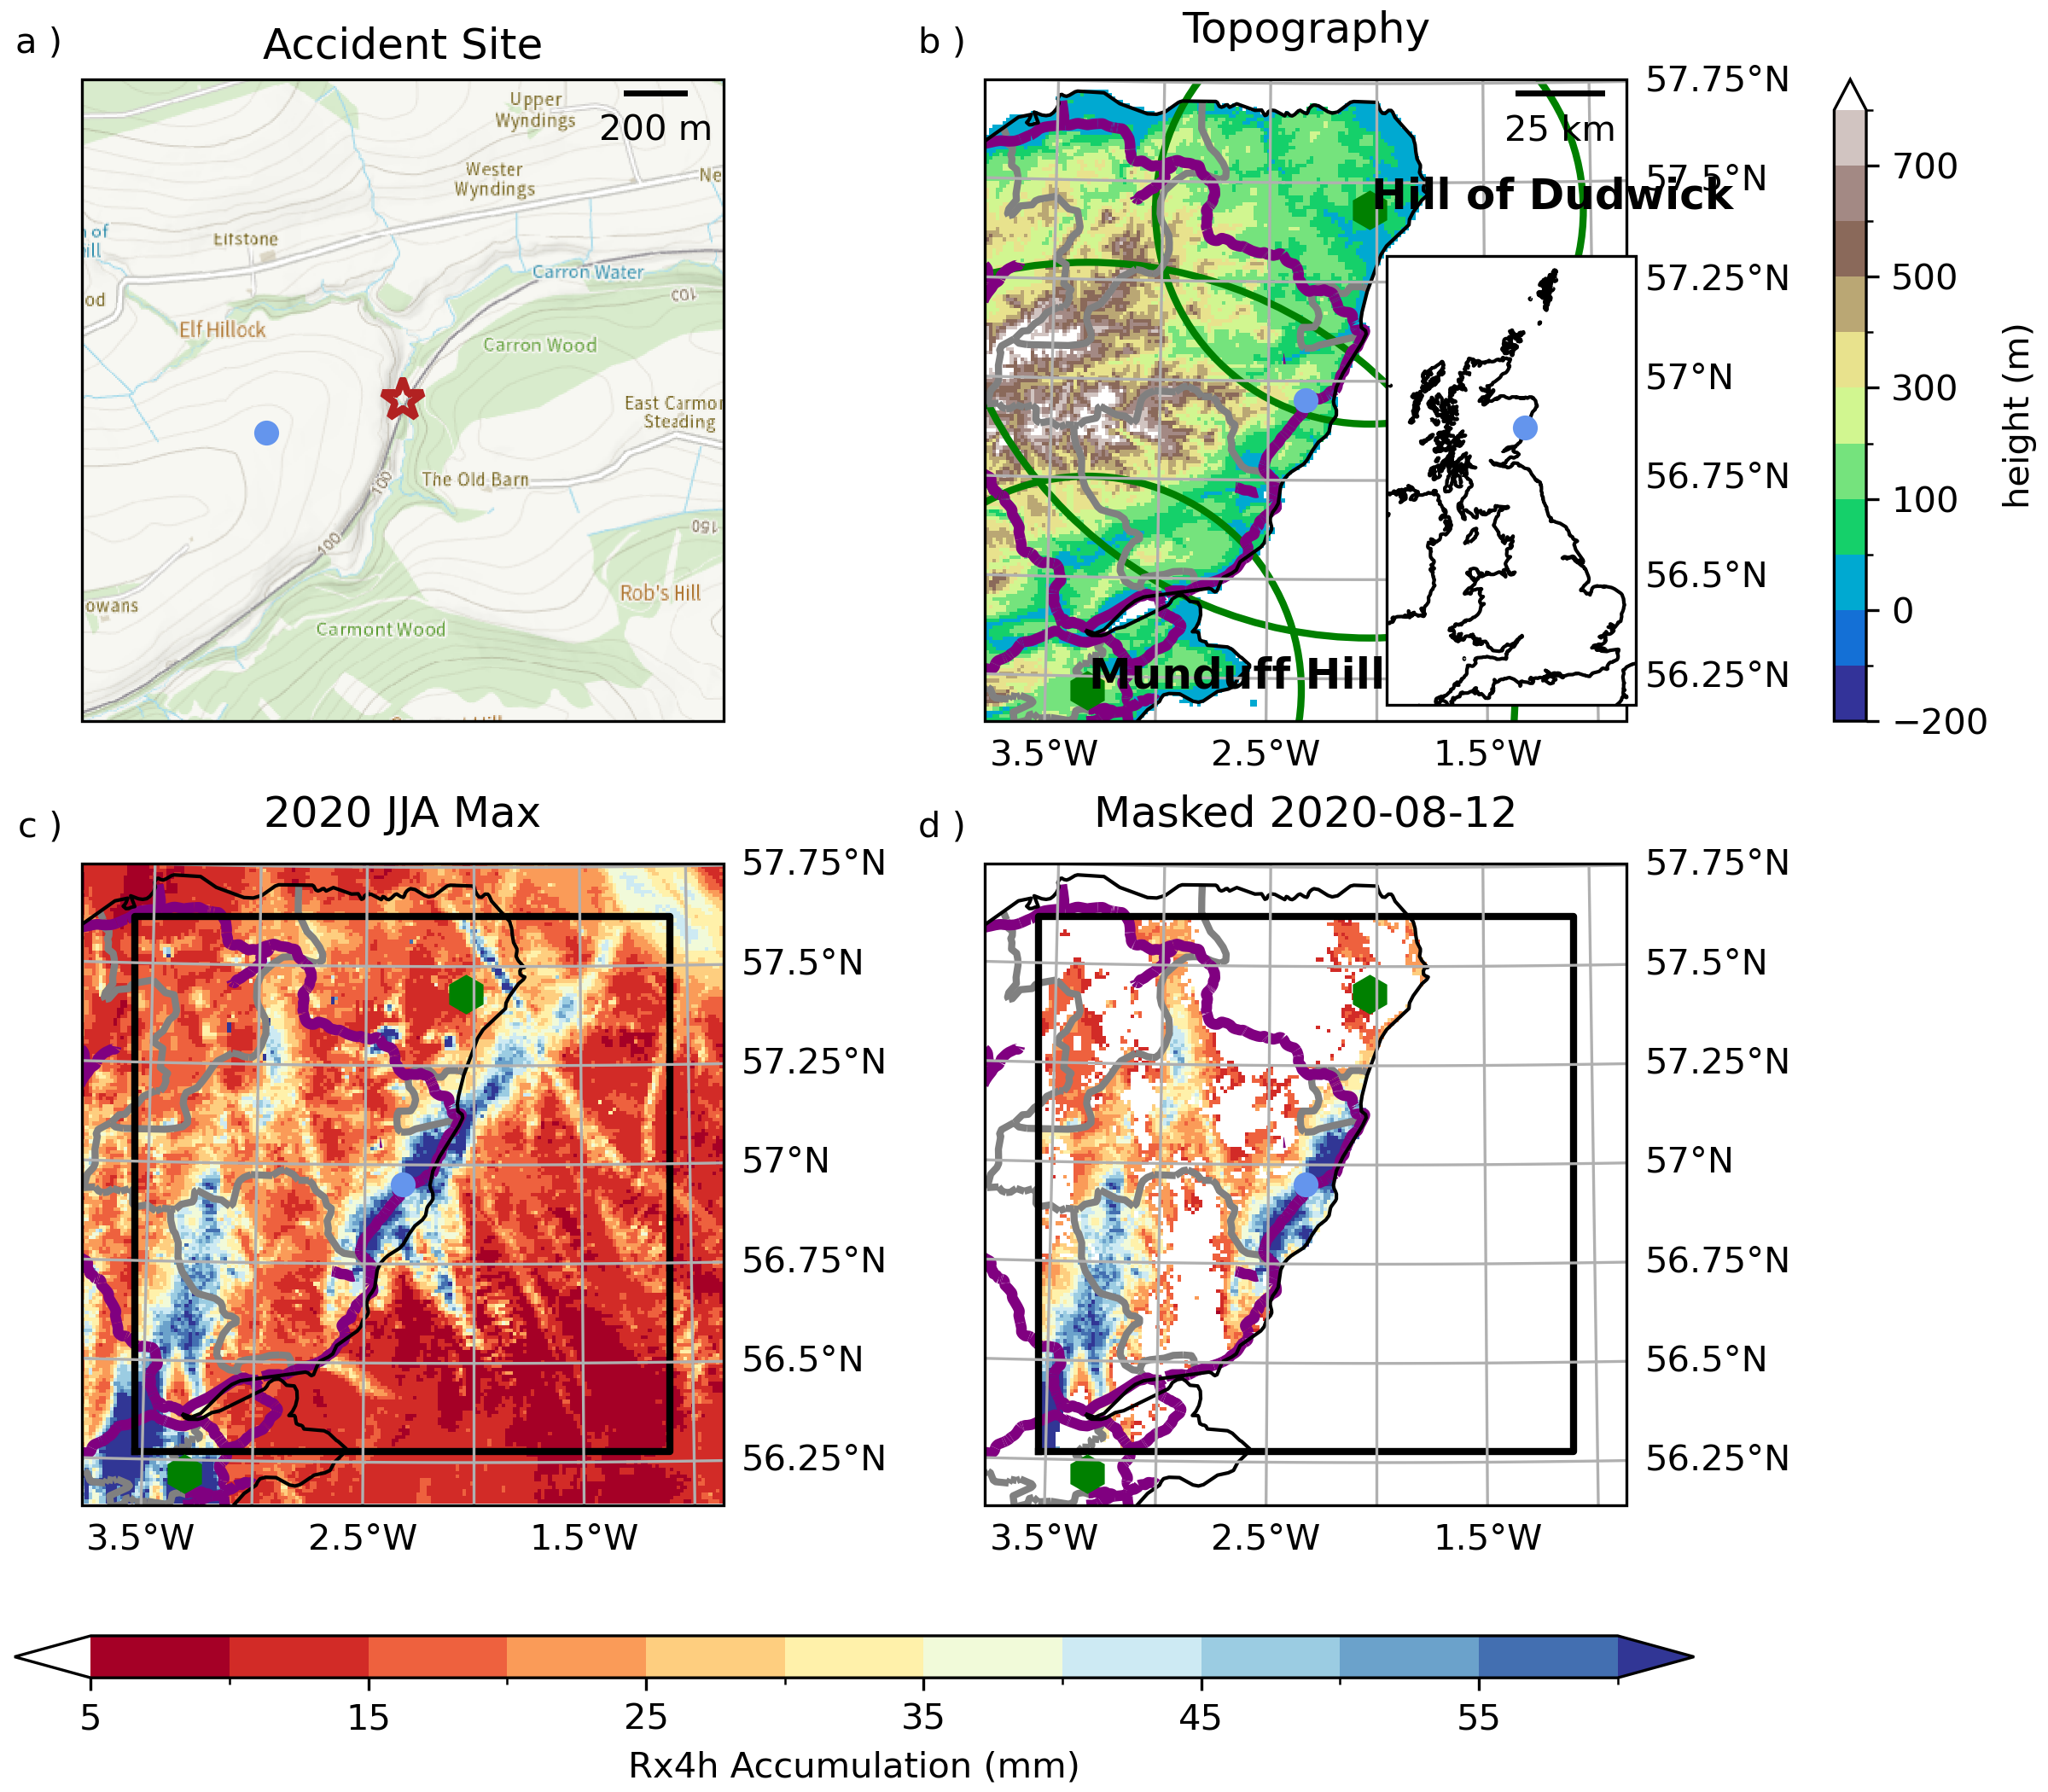
\includegraphics[width=\linewidth]{carmont_geog_group}
	\caption{a) Topography of North East Scotland (at 1km resolution). Also shown, by their first two letters, are locations of Dyce, Aviemore, Aberdeen, Stonehaven and Montrose. Inset shows Great Britain and Ireland. Colour scale on bar to right. Circles are  60 and 120 km from radar stations (green hexagons with full names). b)  Map of Carmont Accident site -- brick red star shows where train derailed. Main features are contour lines every 10 meters, railway (black line) and woods (green) (Map crown copyright Ordinance Survey).  c) Maximum 4 hour radar rainfall accumulation  for JJA 2020. d) Event of 2020-8-21.  Black box in c \& d shows 150x150 km region of interest. Scale bars are shown in a and b. Location of Carmont drain shown in all plots as pale blue dot.  }
	\label{fig:carmont_geog_group}
\end{figure}
\clearpage
\begin{figure}[ht!]
	\centering
	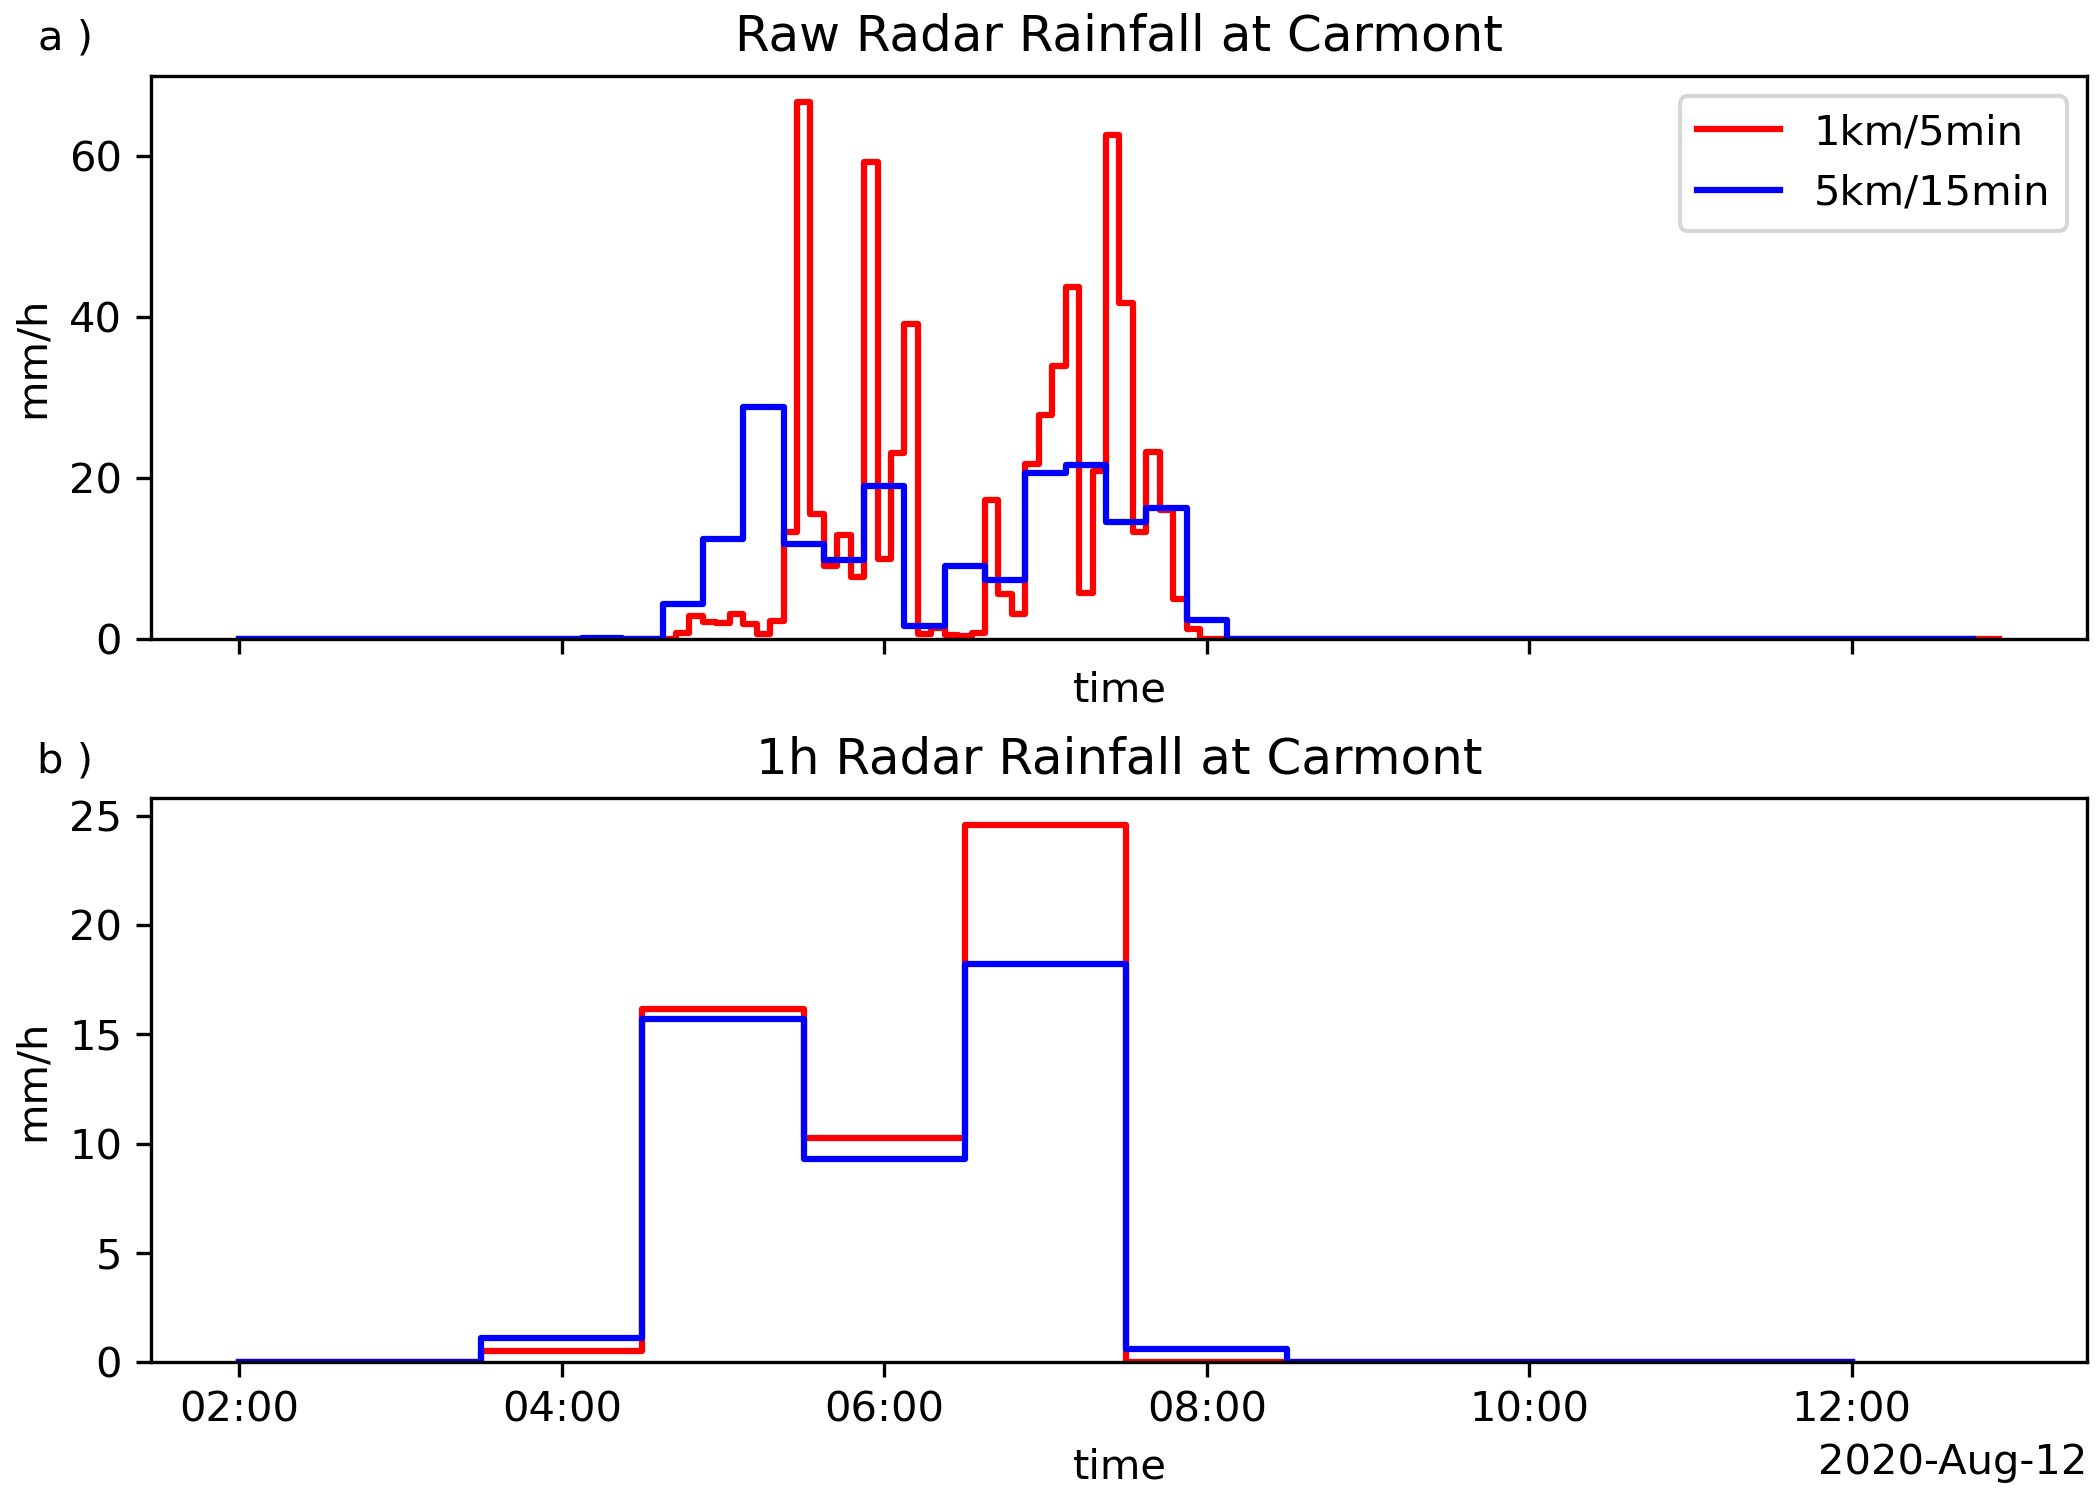
\includegraphics[width=0.5\linewidth]{radar_carmont}
	\caption{a) Radar rainfall rates at Carmont (mm/h) for 1km/5 min (red) and 5km/15 min. Dotted lines show accumulation reaching 51.5 and 44.9 mm for the 1km \& 5km data respectively. Circles show when 1/2 the total rain has fallen; b) Hourly mean rates for 1km (red) and 5km (blue) radar data. Data is shown from 2020-08-12T02:45 to 10:15 and ``Derail'' shows when the train derailed. }
	\label{fig:aug2020_rain}
\end{figure}

\begin{figure}[ht!]
	\centering
	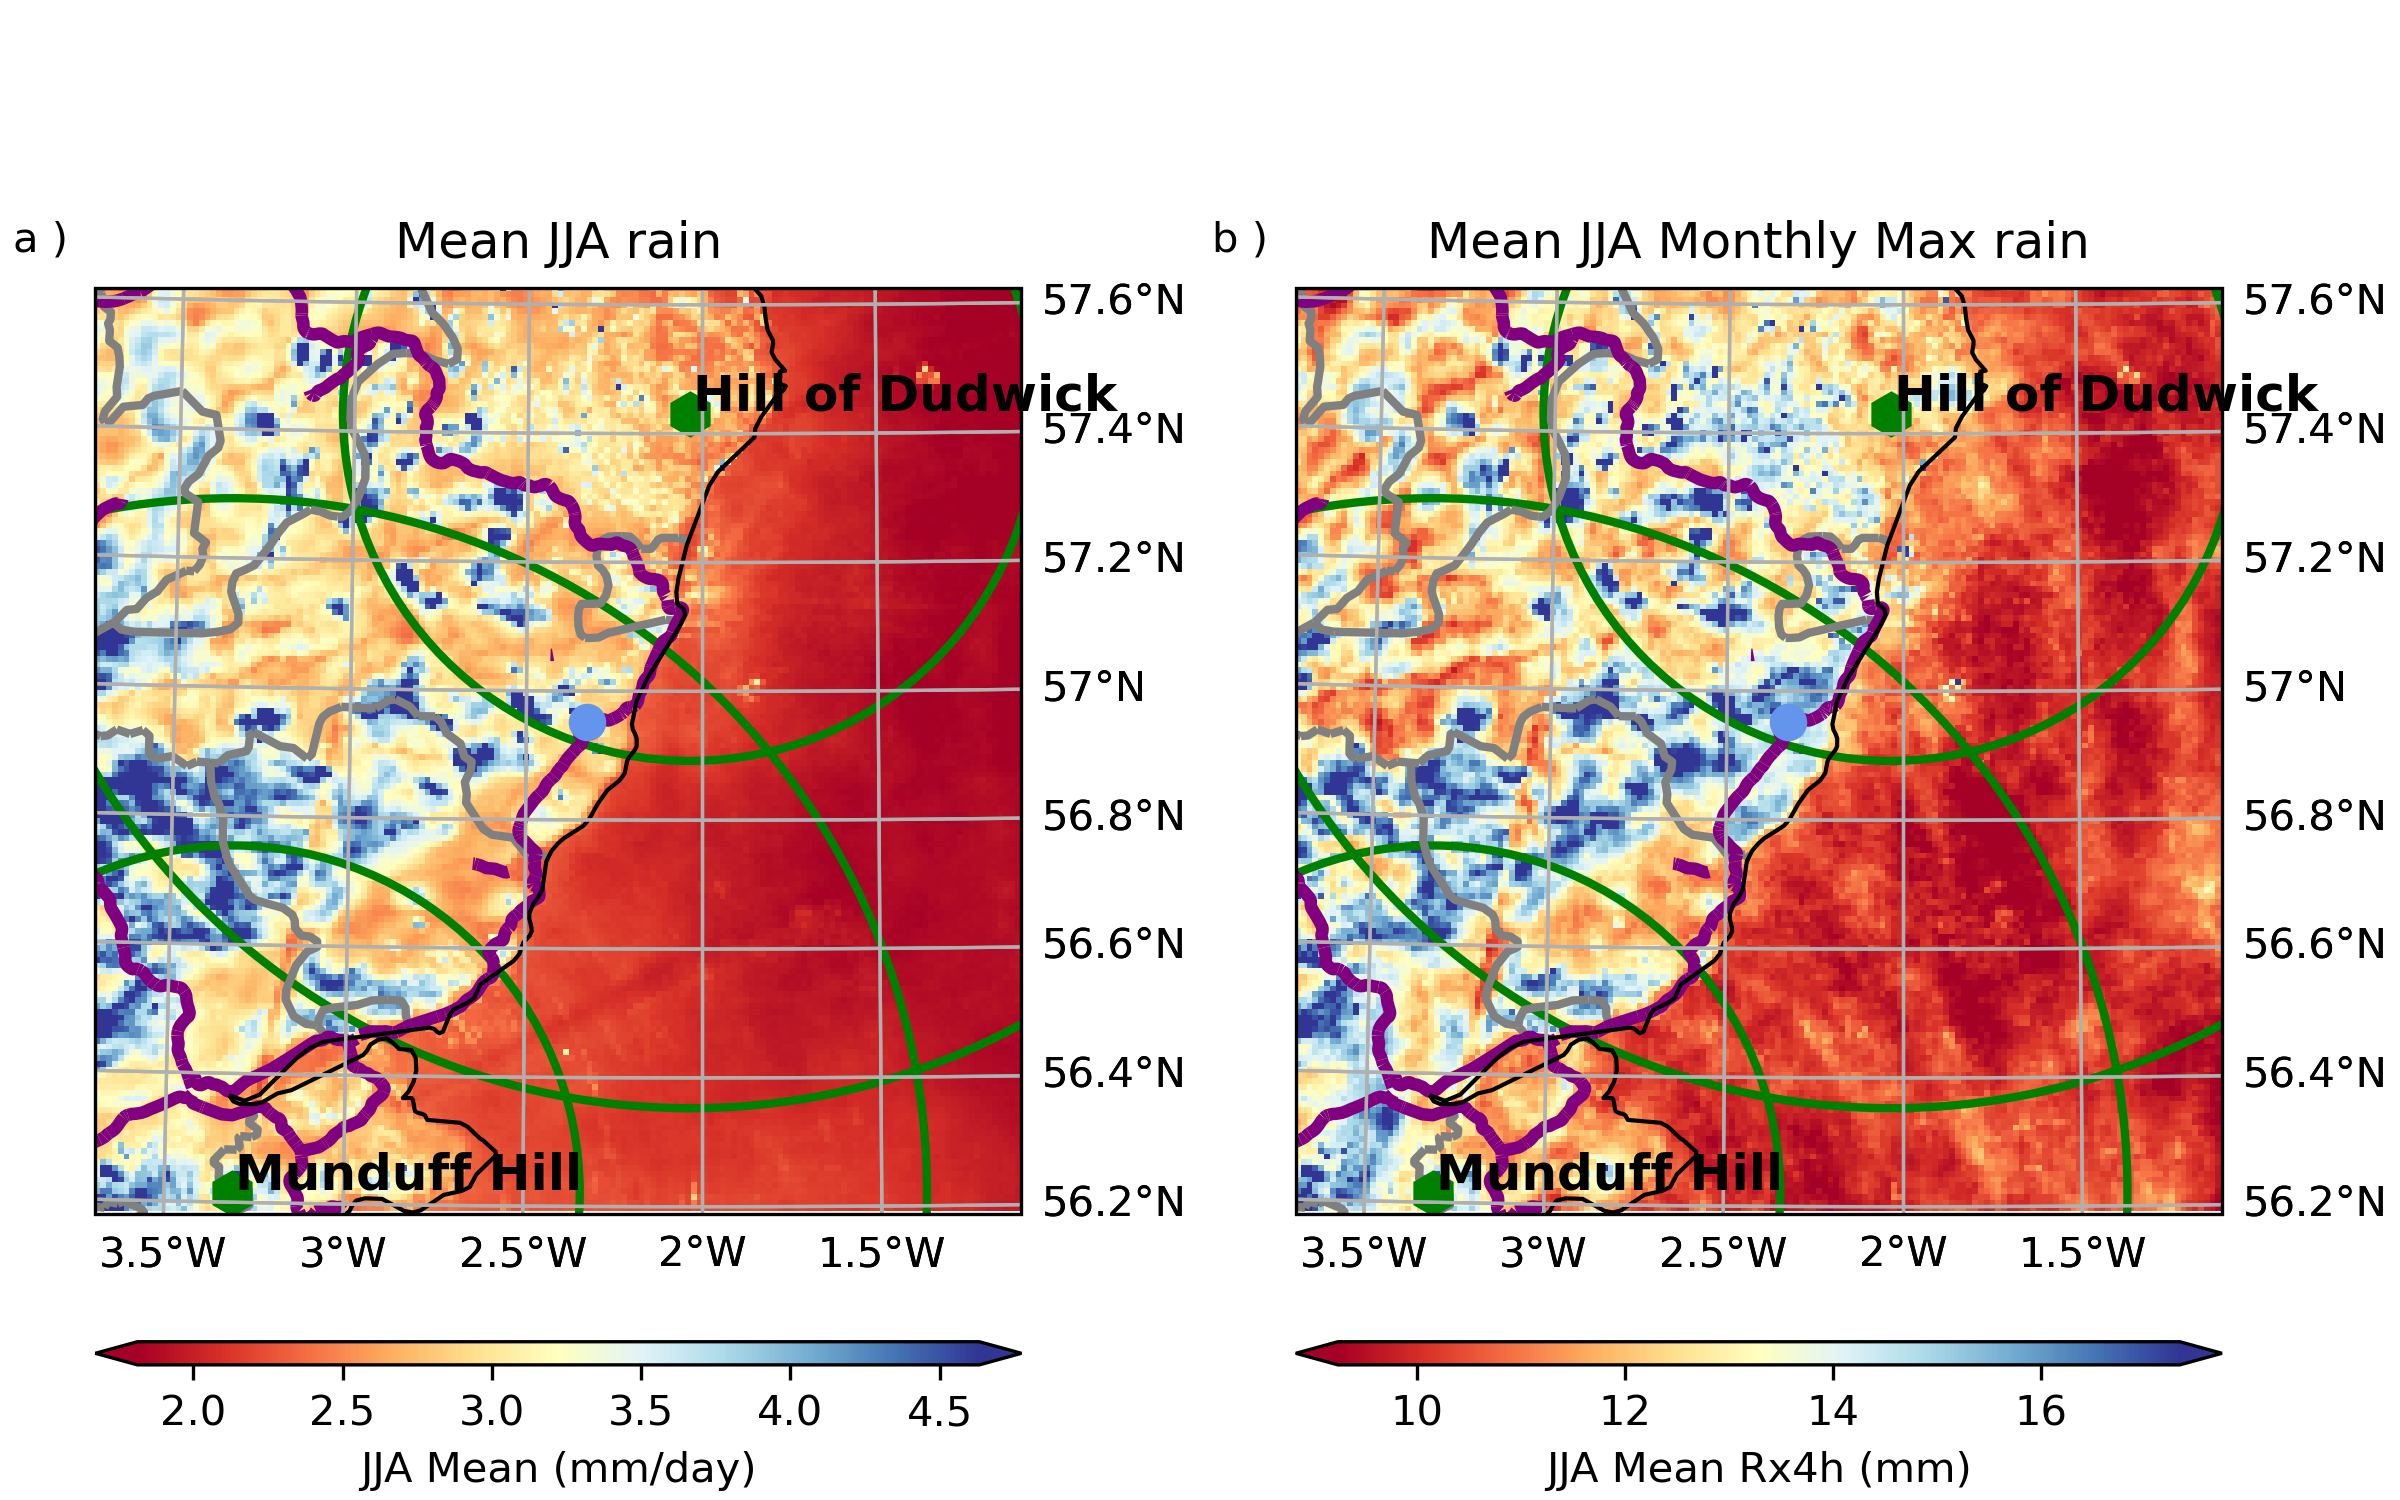
\includegraphics[width=\linewidth]{radar_jja}
	\caption{a) Mean radar rainfall (mm/day) b) Mean monthly maximum 4h rain total (mm/h). Means are for summers (June-July-August) from 2008 to 2023 inclusive. Circles are  60 and 120 km from radar stations (Green hexagons). Pale blue circle shows point ("Carmont drain") where rain occurred, purple lines show railways and grey lines local authority boundaries. Semi-transparent green lines (circles) show radial features (localised sources) which may be radar artefacts. }
	\label{fig:radar_jja}
\end{figure}


\begin{figure}
	\centering
	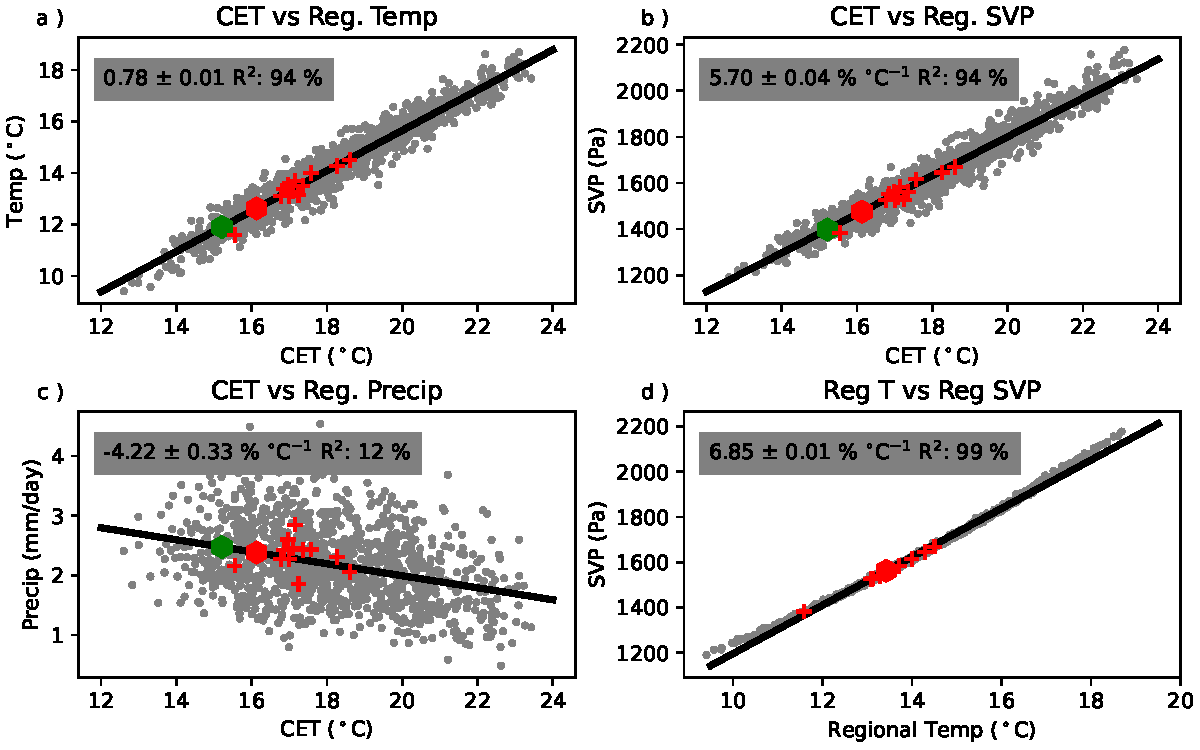
\includegraphics[width=\linewidth]{scatter}
	\caption{Scatter plots for summer mean  a)  Central England Temperature (CET) vs  regional mean temperature; b) CET vs regional average saturated vapour pressure (SVP); c) CET vs regional average precipitation; d) Regional temperature vs Regional SVP. In all plots green and red hexagons show estimated 1850-1899 and 2012-2021 average values using regression predictions from observed CET values. Lines show linear best fits. Red crosses show, for each ensemble, mean simulated values for 2008-2023. Text shows  change, and standard error, for  $1^{\circ}C$ change in CET or Regional Temperature, and $R^2$ of fit.}
	\label{fig:cet_scatter}
\end{figure}

\begin{figure}
	\centering
	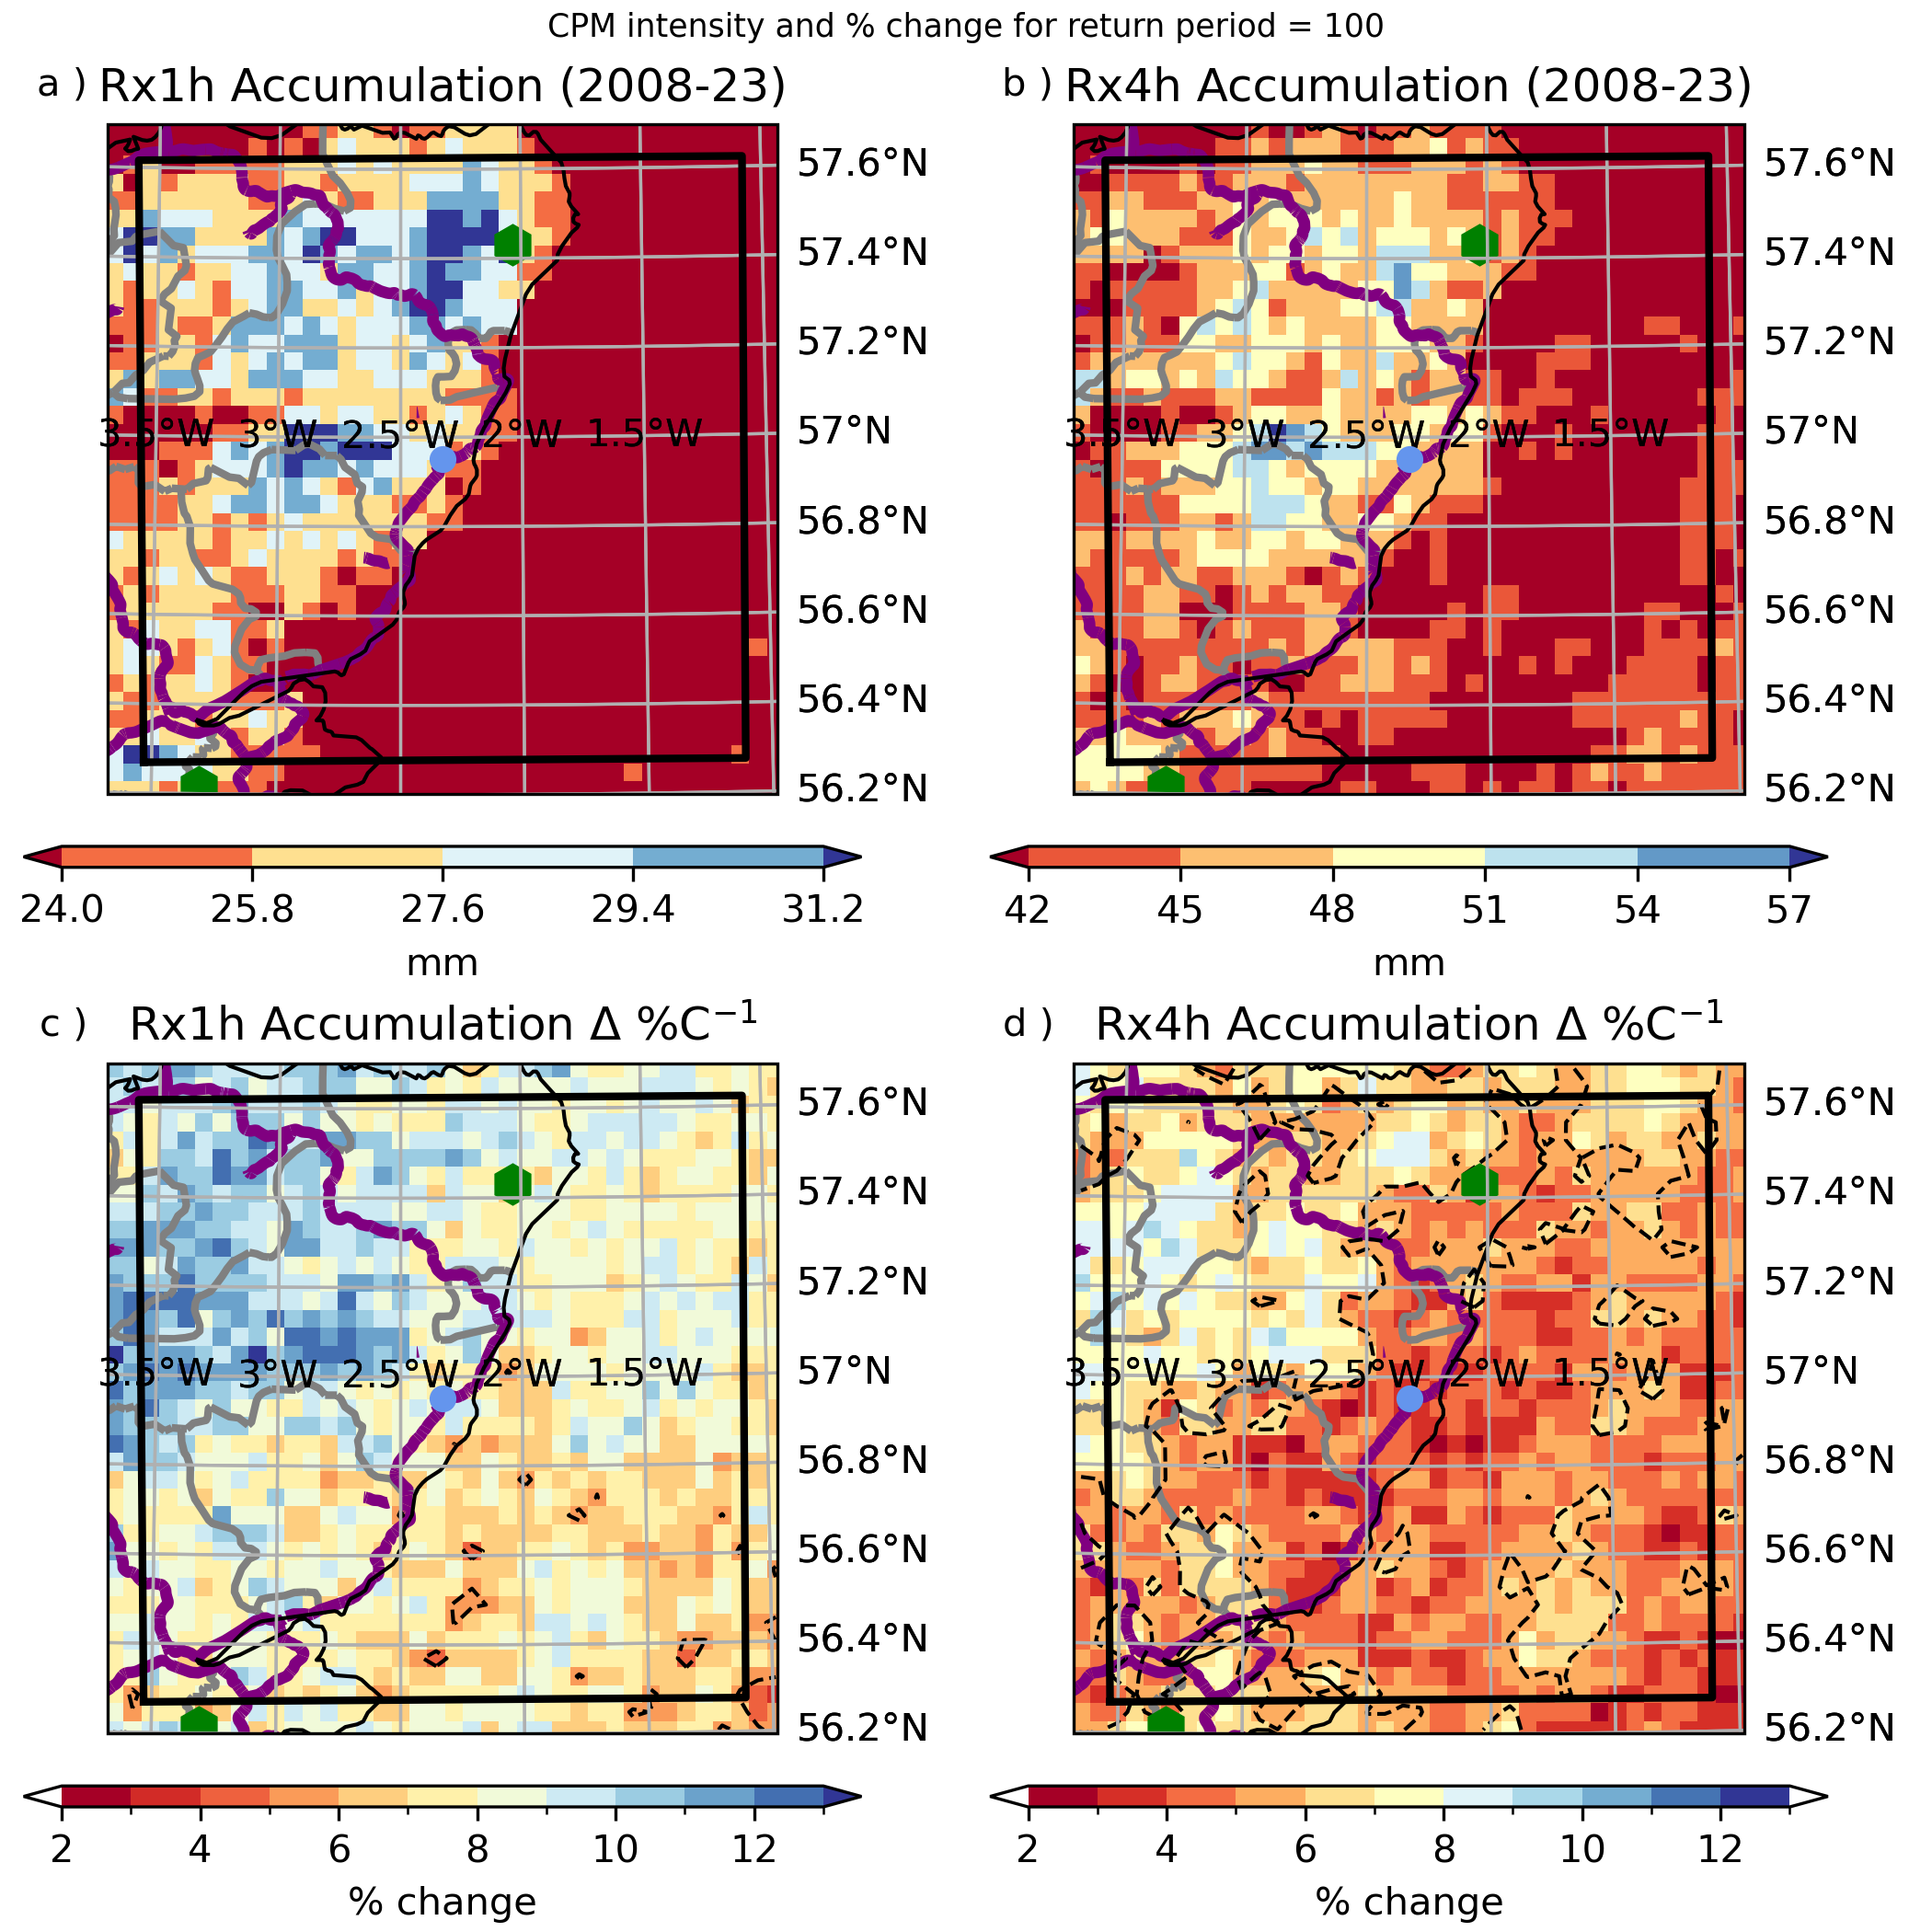
\includegraphics[width=1\linewidth]{cpm_intensity_delta}
	\caption{One in a hundred year CPM maximum rainfall accumulation for 1 and 4 hour rainfall (a \& c) and percentage sensitivity to 1 degree CET increase. Accumulation (a \& c) colour table levels are $\pm$ 15\% of the values at Carmont Drain. Dashed lines (b \& d) shows intensity increase of 5.7\%/degree CET corresponding to CC. Other elements as Figure~\ref{fig:radar_jja}.  }
	\label{fig:map_intensity}
\end{figure}

\begin{figure}
	\centering
	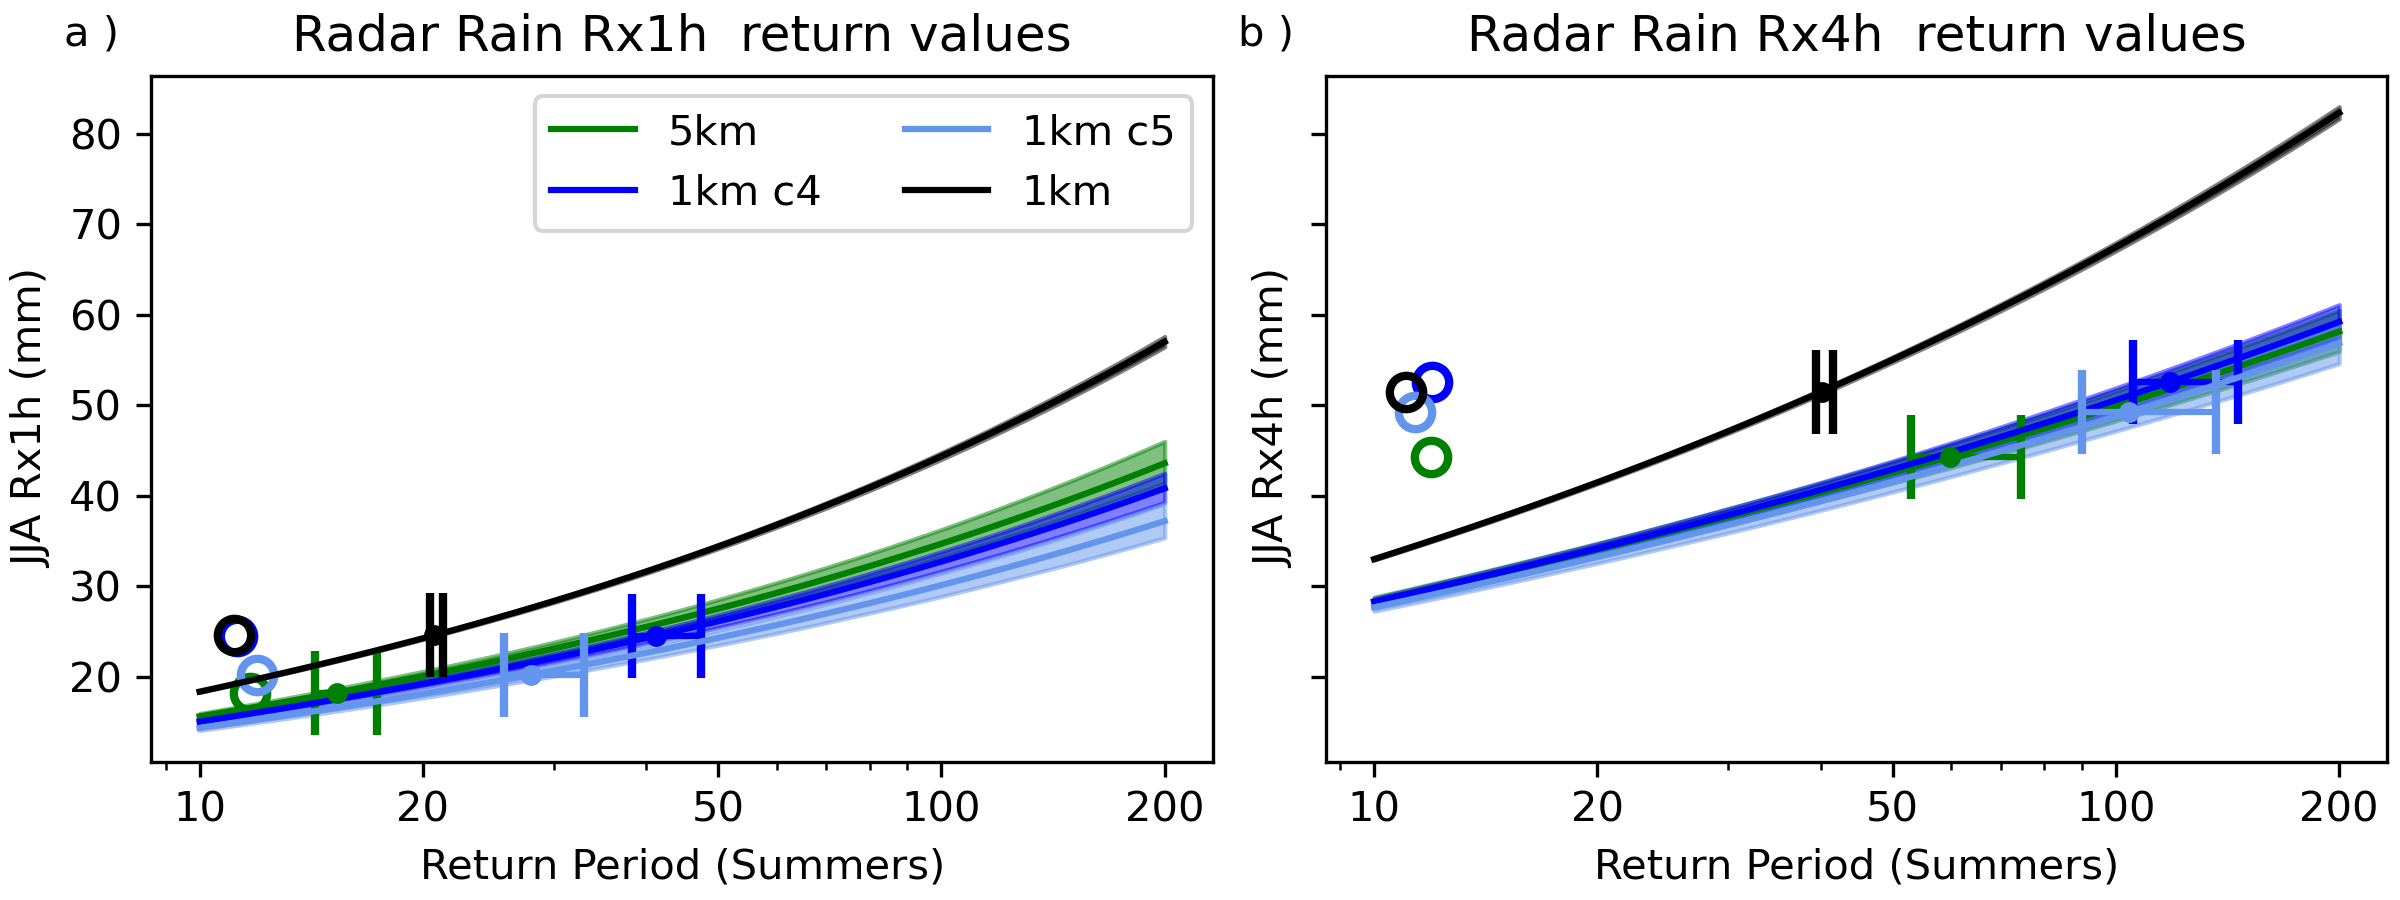
\includegraphics[width=\linewidth]{radar_return_prds}
	\caption{Estimated return values for  JJA maximum accumulated radar rainfall. Shown are Rx1h (a) and Rx4h (b) for 1km  (black),  5km (green), 1km-c4 (blue) and 1km-c5 (pale blue) radar rain. Symbols in left hand of sub plots show radar rain at nearest gridpoint to Carmont drain. Horizontal error bars show 5-95\% return period uncertainty ranges. }
	\label{fig:radar_rtn_prd}
\end{figure}

\begin{figure}
	\centering
	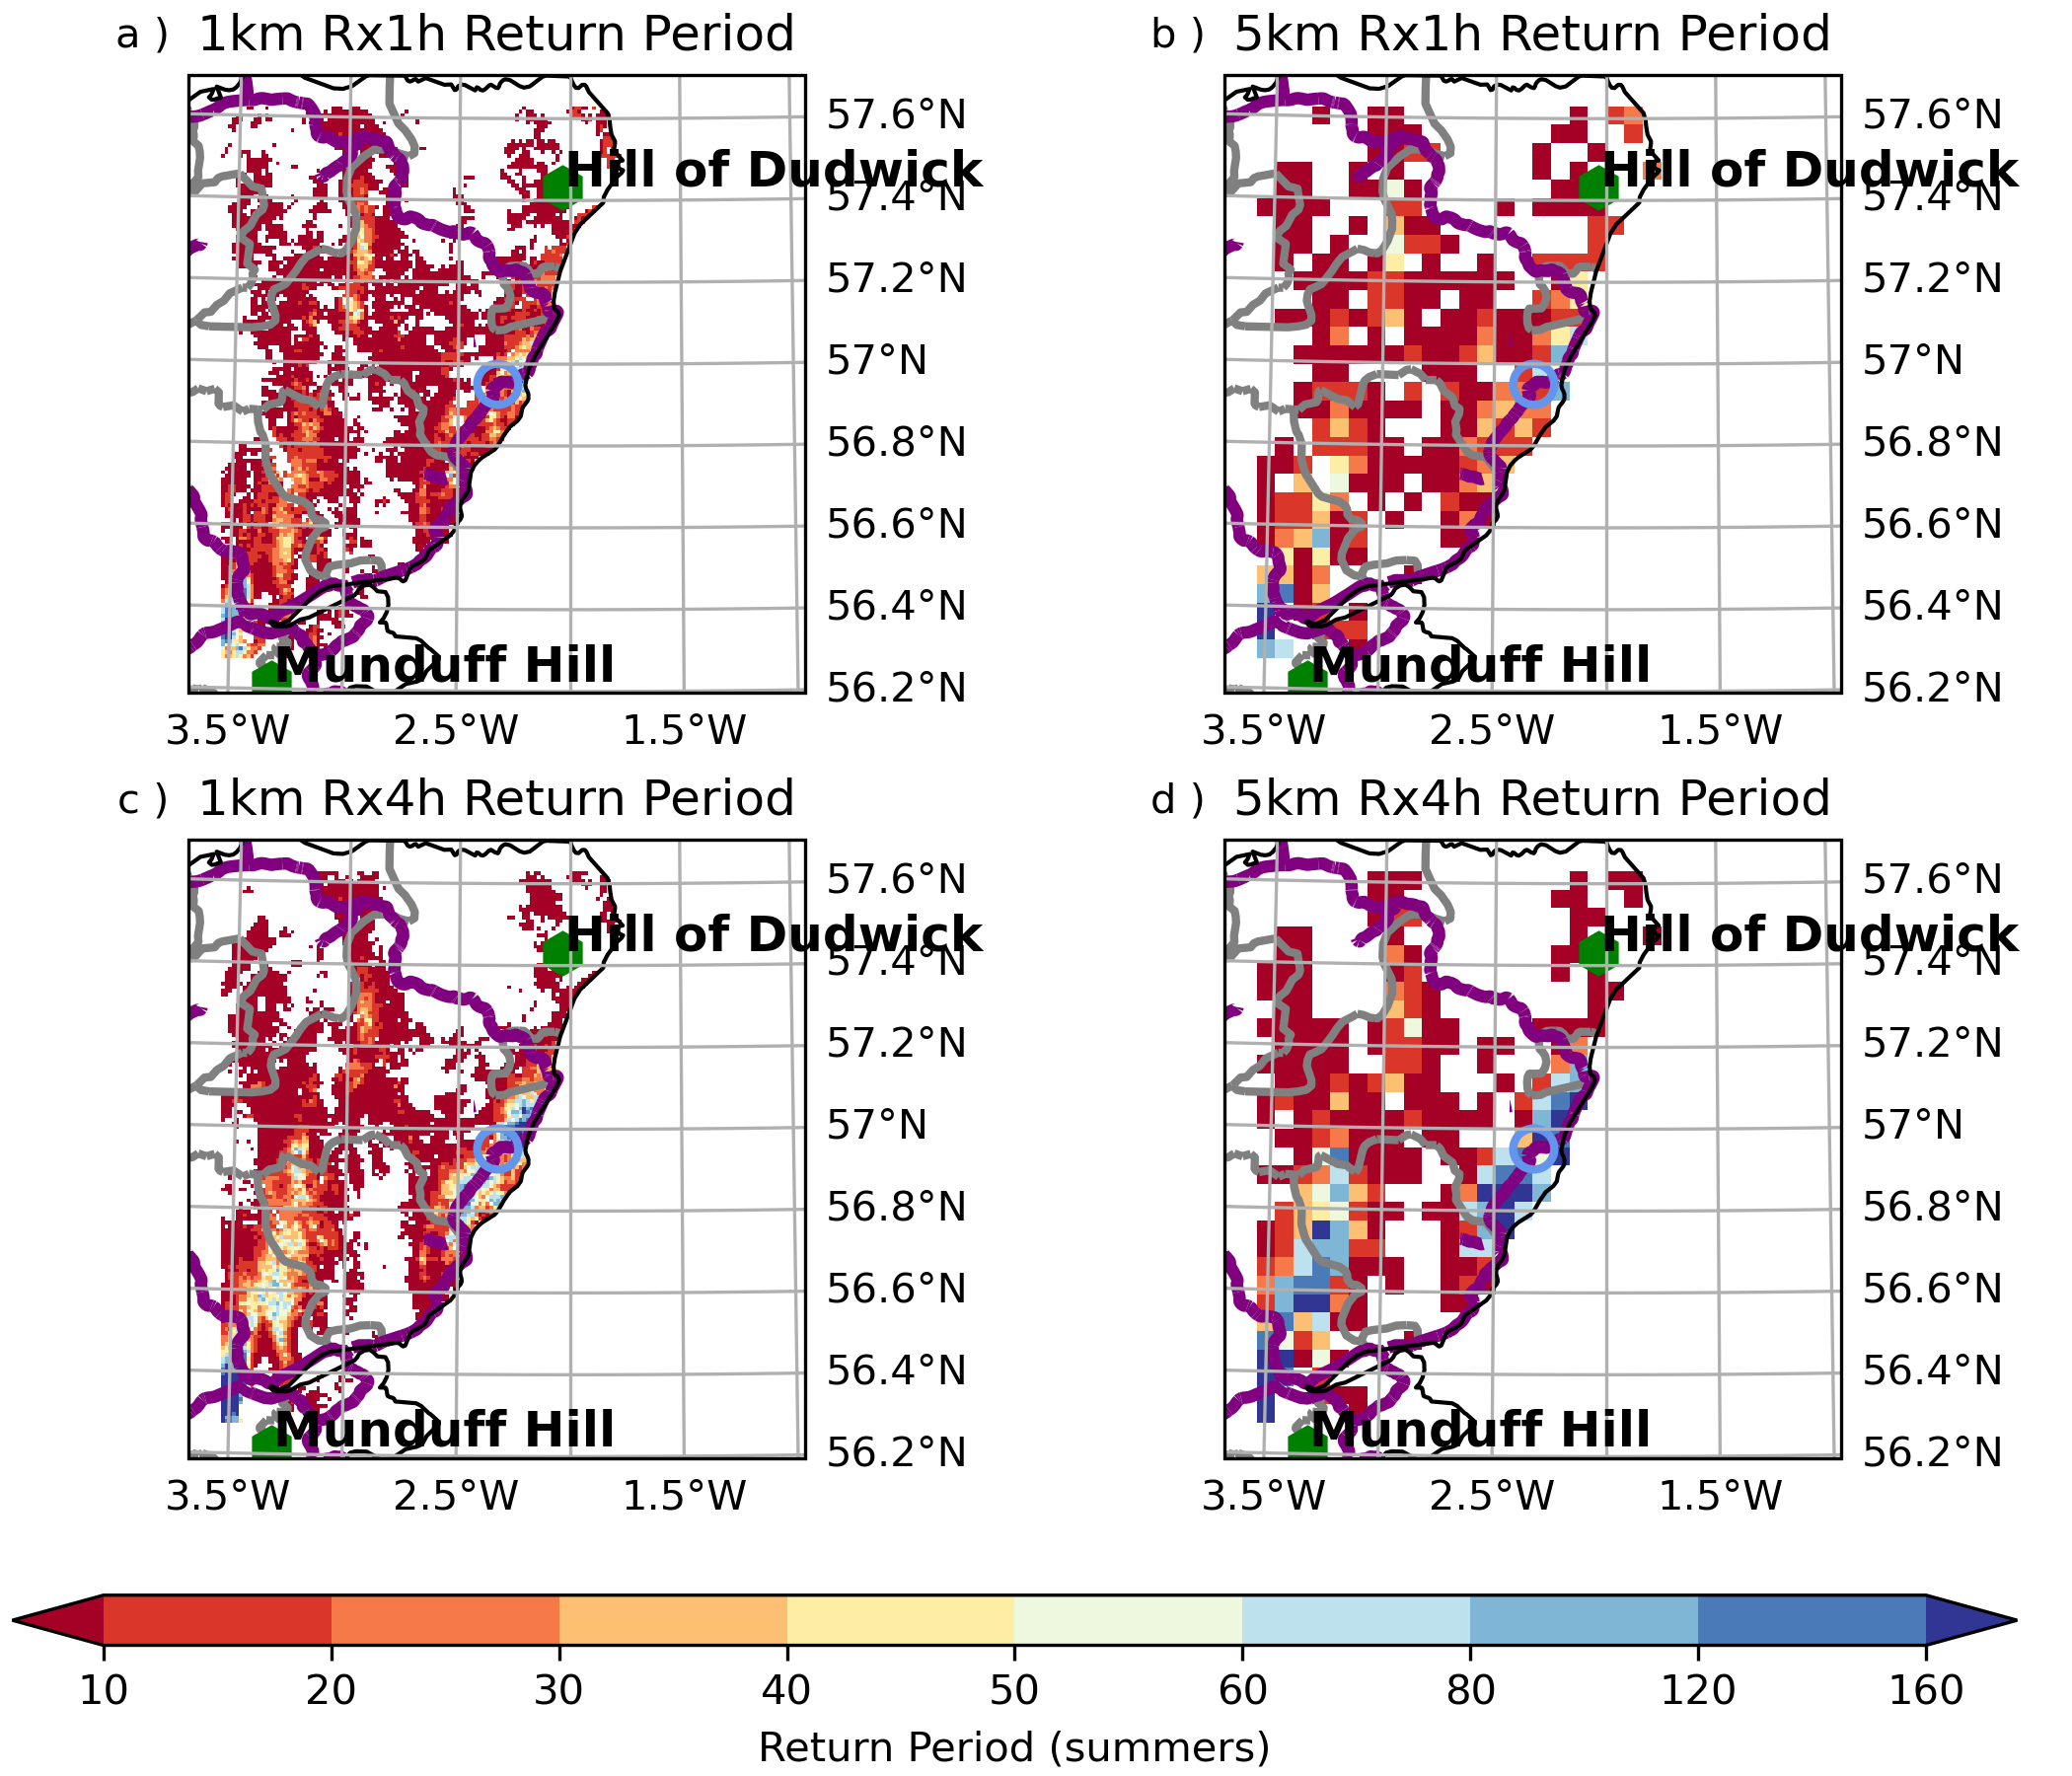
\includegraphics[width=\linewidth]{map_return_prds}
	\caption{Return periods for Carmont regional Rx1h and Rx4h accumulations which occurred on 2020-08-12. Plots a \& b show Rx1h while plots c \& d show Rx4h. Color bar at bottom refers to all plots. Other elements as Figure~\ref{fig:radar_jja}. } 
	\label{fig:map_rtn_prd}
\end{figure}


\begin{figure}
	\centering
	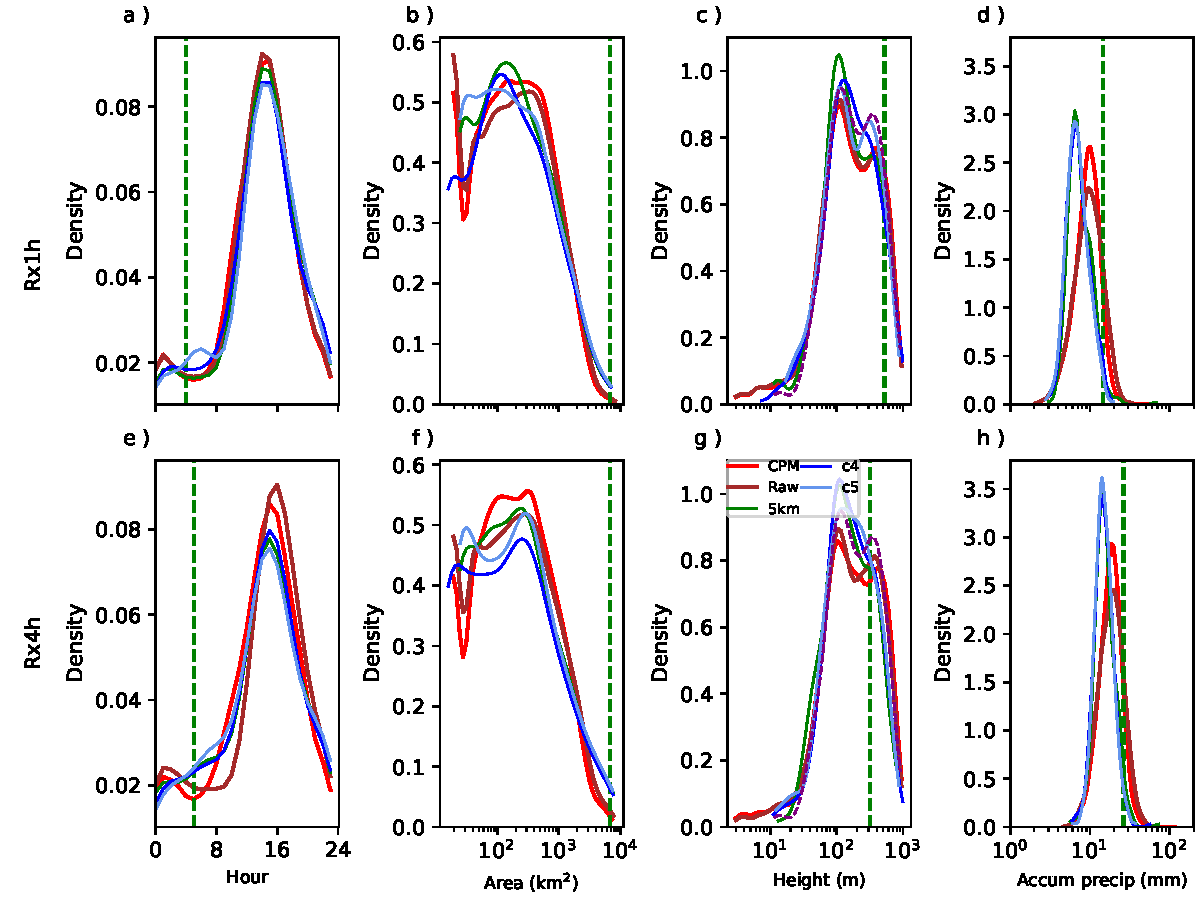
\includegraphics[width=\linewidth]{kde_smooth_events}
	\caption{Kernel Density Estimates (KDE) from  CPM (orange), CPM-Raw (brown), 5km radar (green), 1km-c4 (blue) and 1km-c5 (pale blue) events at 50\% quantile for 2008-2022 period.
		 Shown are day-hour (a \& e),$\log_{10}$ of event area (b \& f),  topographic height (c \& g ) and maximum Rainfall accumulation (d \& h).
		  Top row shows Rx1h while bottom row shows Rx4h values. Shown in c \& g is the KDE for the 5km DEM topography. Vertical green lines shows values of 2020-08-12 for 5km radar dataset.}
	\label{fig:kde_smooth_events}
\end{figure}

\clearpage
\begin{figure}[ht!]
	\centering
	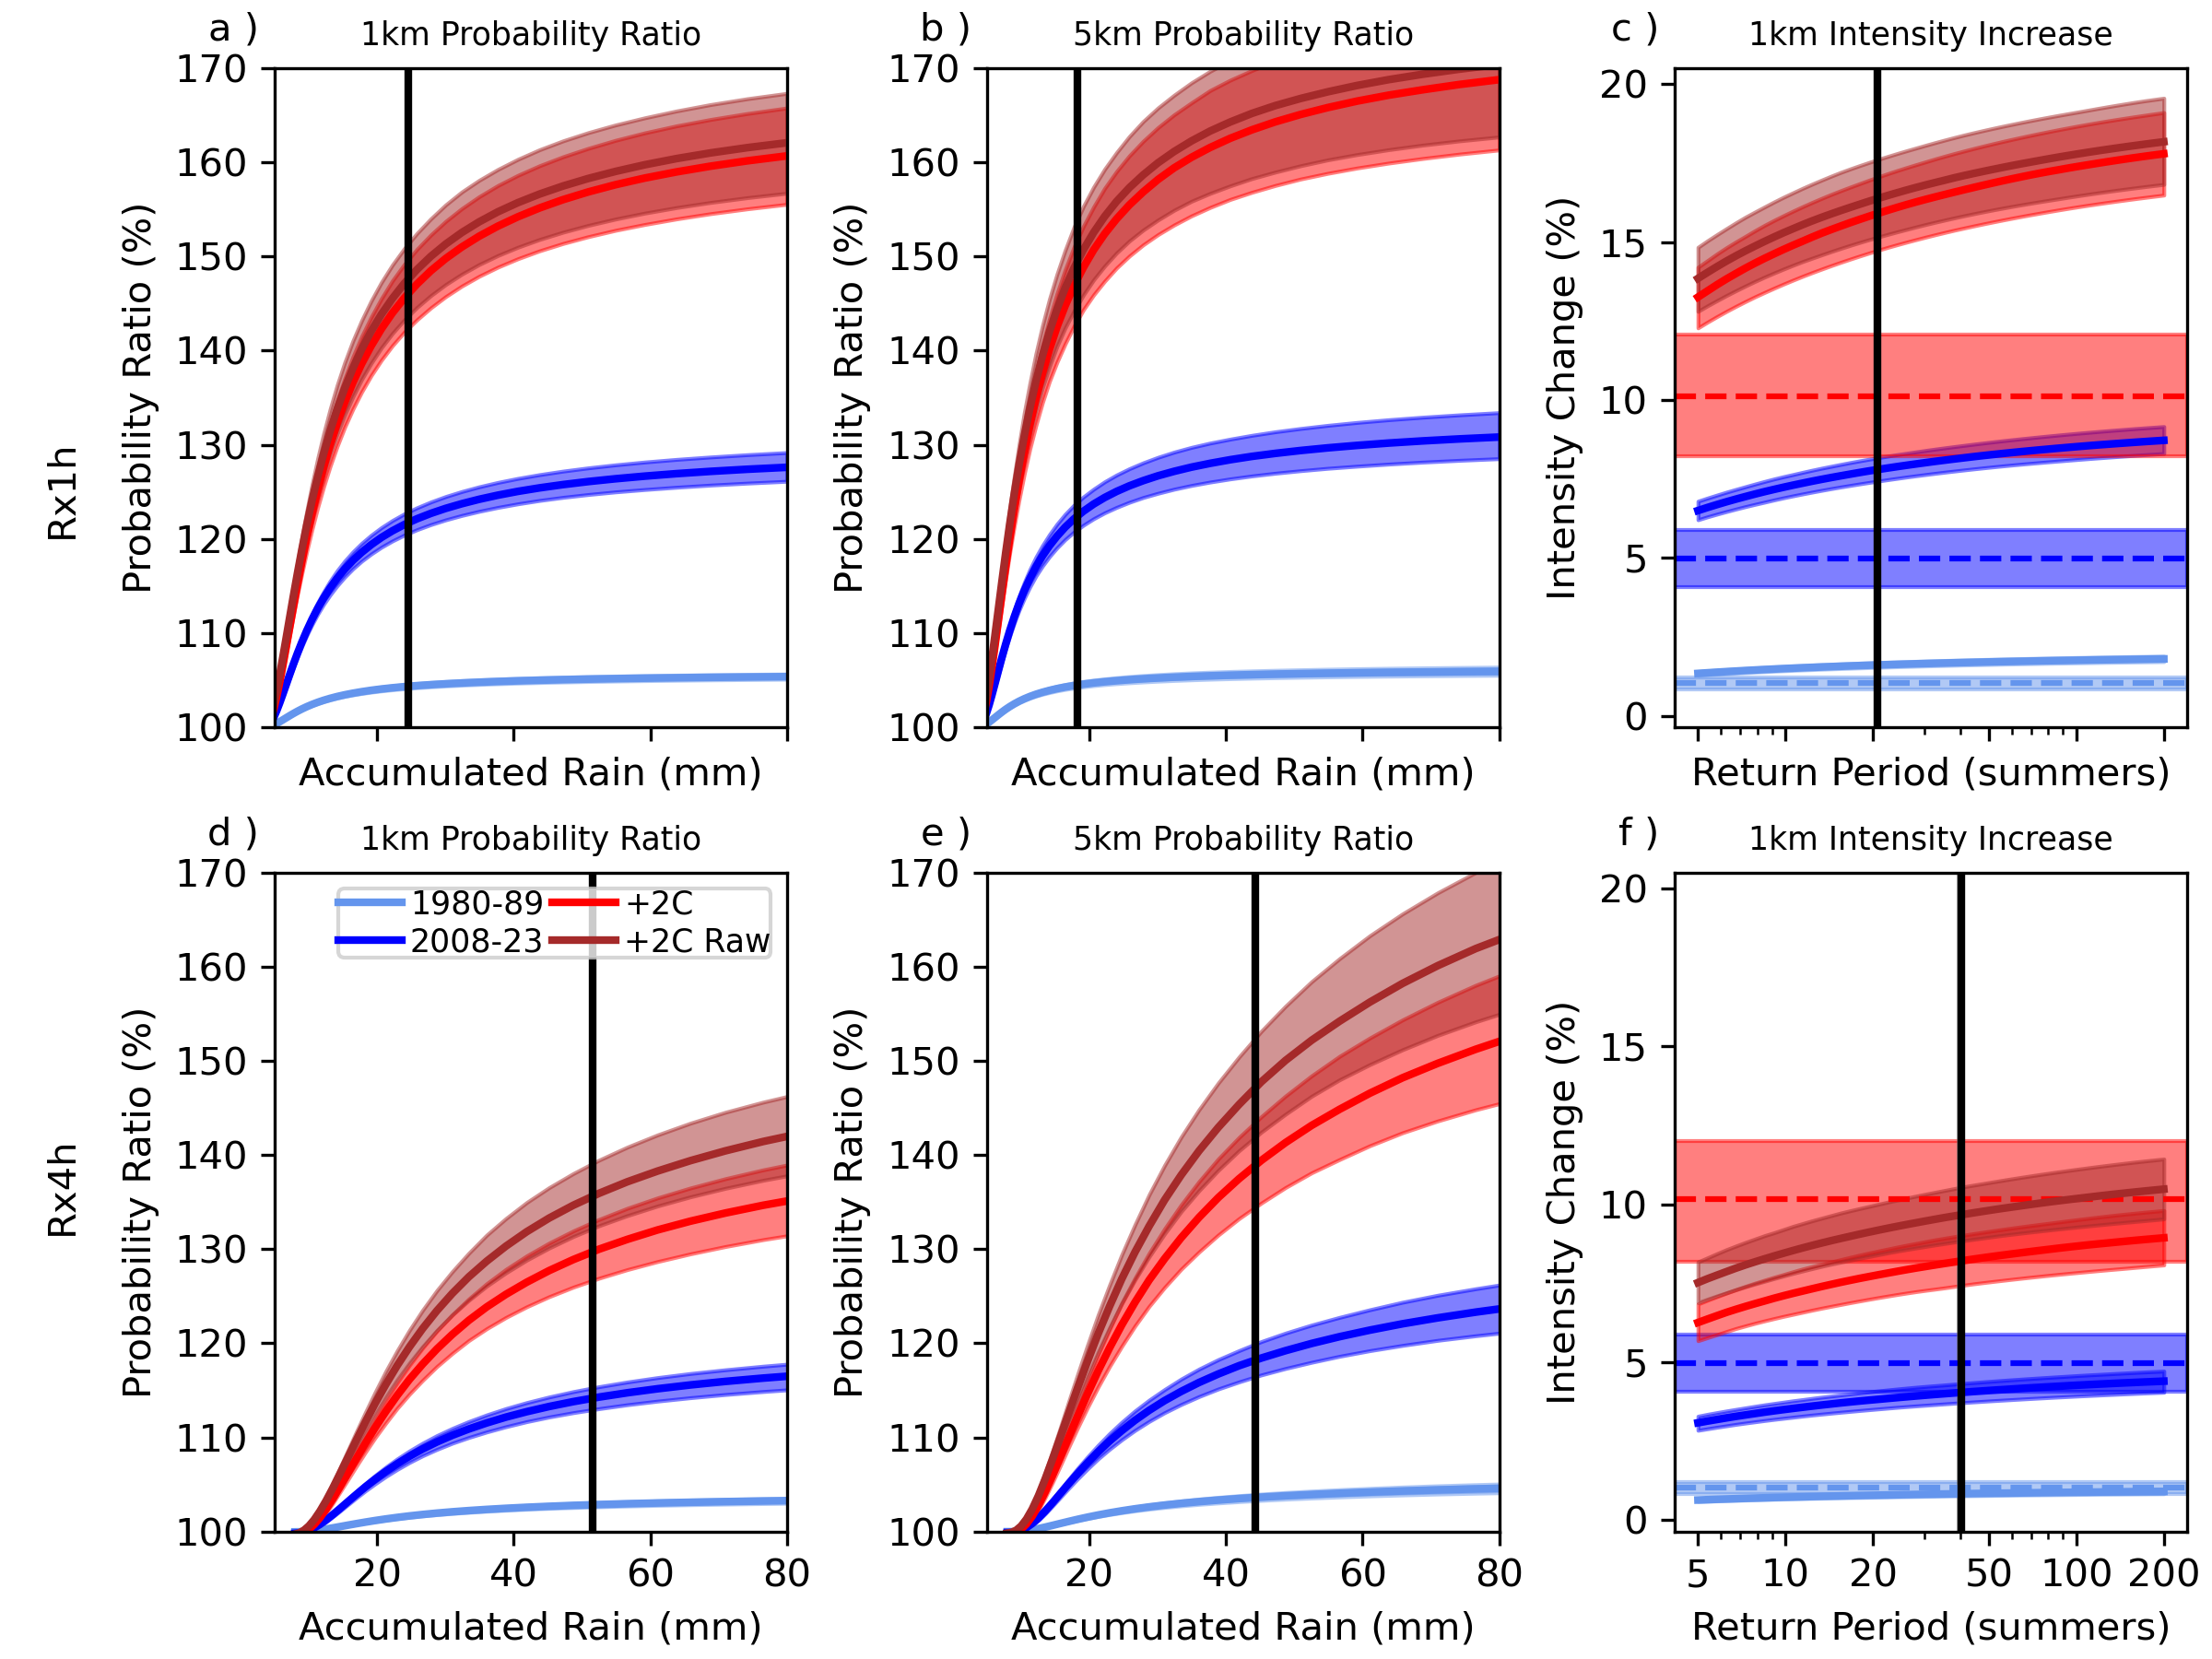
\includegraphics[width=0.9\linewidth]{intens_prob_ratios}
	\caption{a \& d: Probability ratio, relative to Pre-industrial, at Carmont drain as function of accumulated rainfall for 1km radar rainfall. b \& e) As a but for 5km radar rainfall. c \& f: Intensity ratio at Carmont drain  as function of  return period. Also shown are median (horizontal dashed line) and 5-95\% uncertainties (vertical shading) for changes expected from Clausius-Clapyron. Upper plots (a-c) show Rx1h accumulations while lower plots (d-f) show Rx4h accumulations. All plots show changes for +2C world (red), 2012-2021 (dark blue) and 1980-1989 (pale blue) from filtered CPM data. Brown shows changes in +2C world when raw CPM data is used.   Solid lines are median changes with 5-95\% uncertainty range shown by  shading.}
	\label{fig:intense_prob_ratios}
\end{figure}
\clearpage
\begin{figure}[ht!]
	\centering
	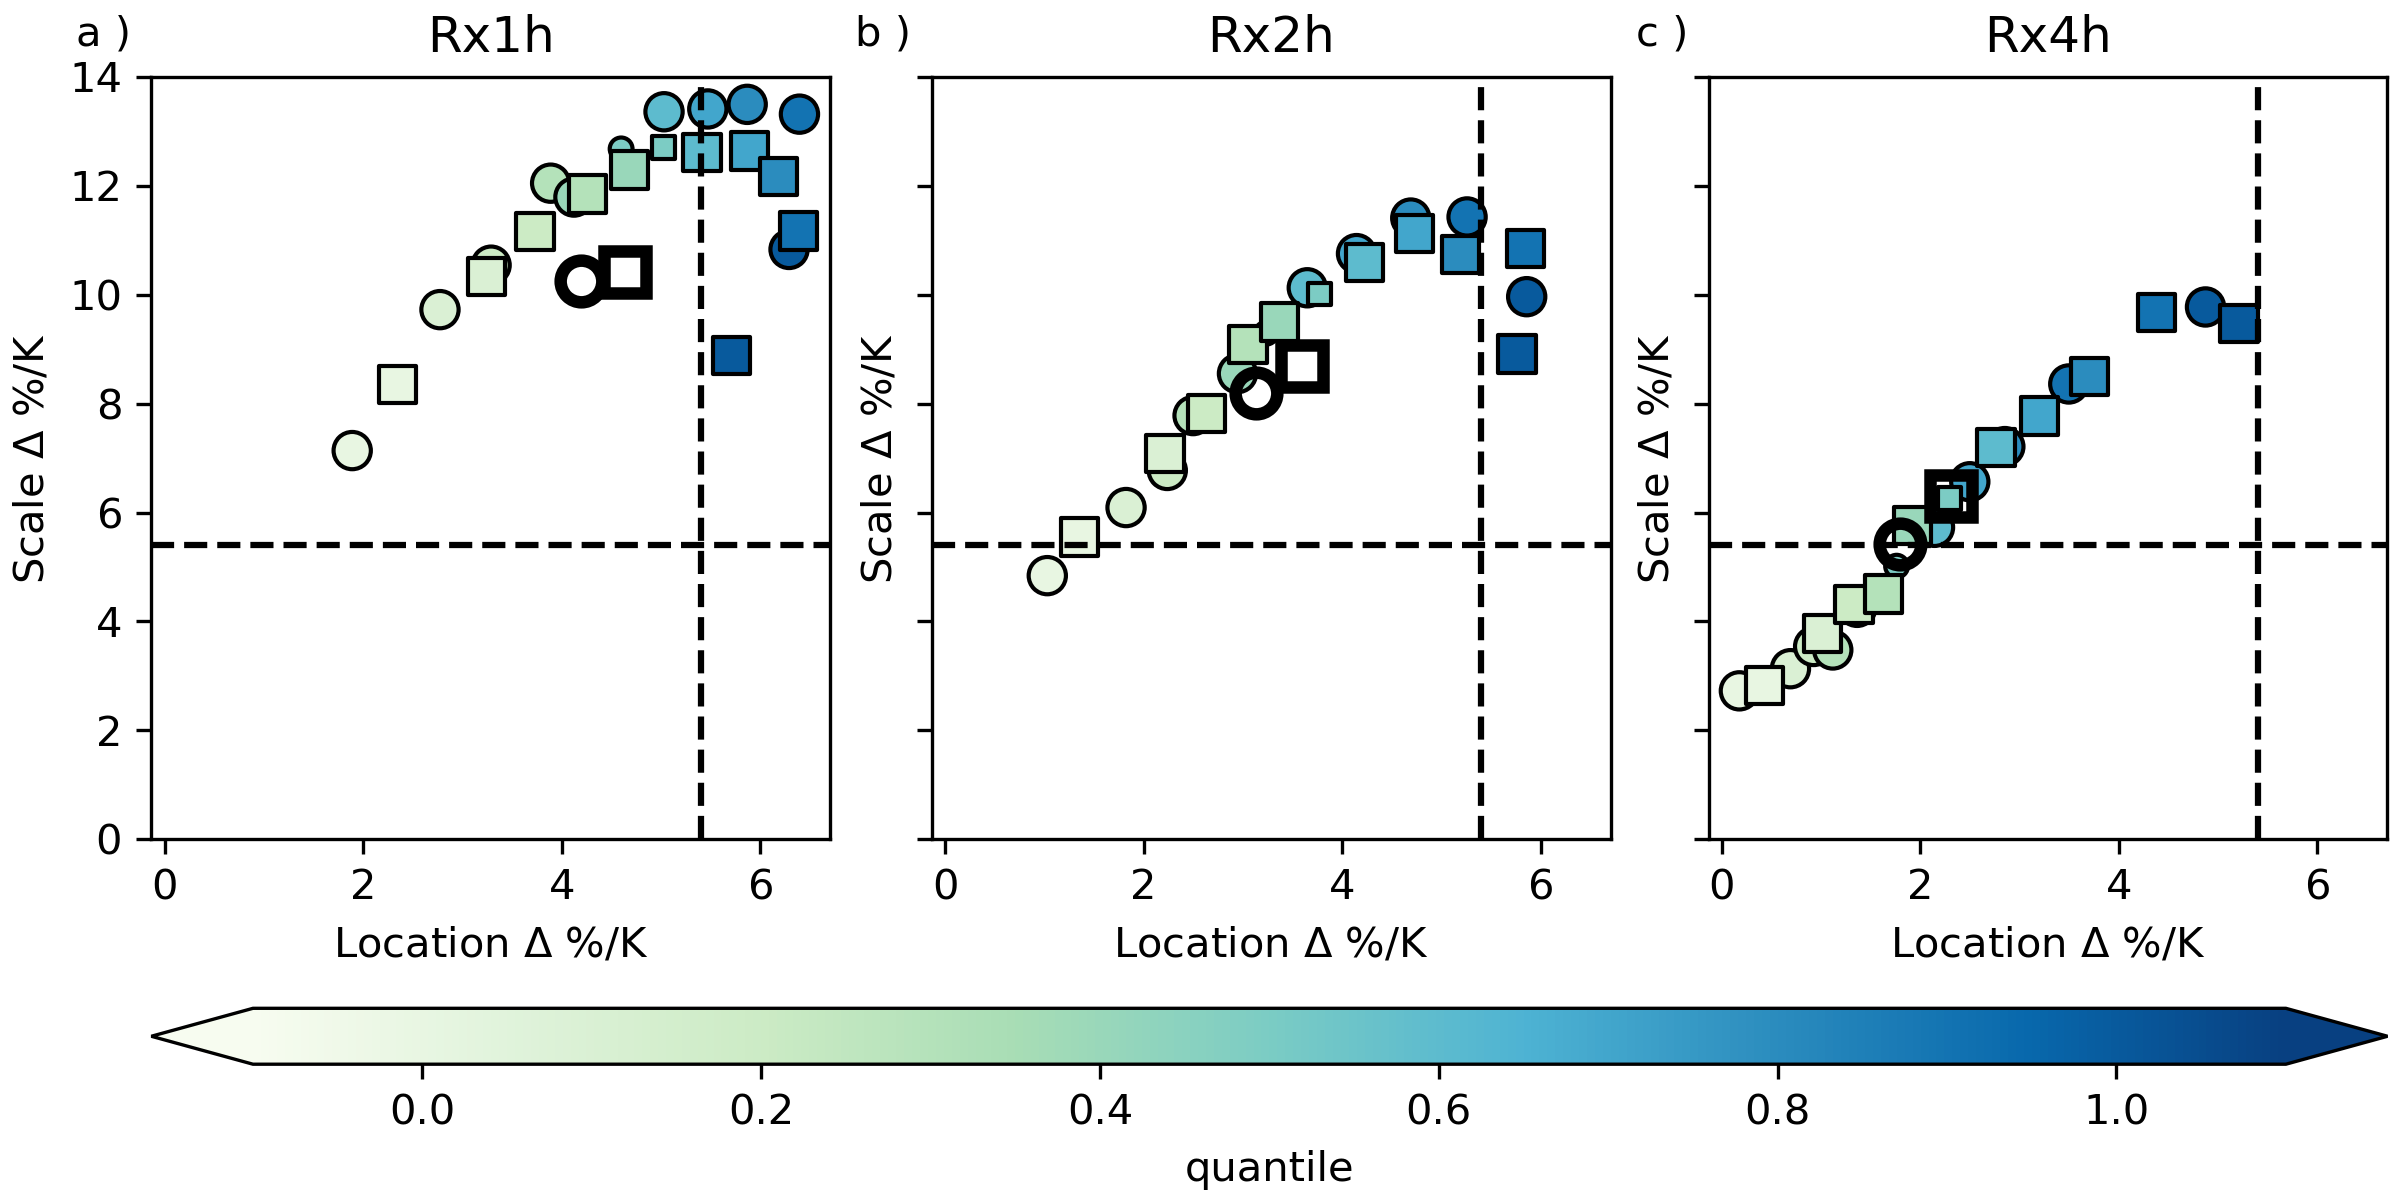
\includegraphics[width=\linewidth]{carmont_gev_quant_change}
	\caption{
		Fractional change in GEV scale  and location parameters for raw (squares) and filtered (circles) CPM data. 
				Colours denote quantiles in 5x5 region (approximately 22x22 km) centred on Carmont Drain. 
				Small symbols show where change is not significantly different from median quantile change.
				Dashed horizontal and vertical lines show mean Clausius-Clapeyron changes.
				Black symbols show fractional change for the whole region.  
				Shown are Rx1h (a), Rx2h (b) and Rx4h values.
	}
	\label{fig:carmont_gev_quant_change}
\end{figure}

\end{document}
